

\chapter{Hash Functions}

\section{Fingerprinting}
	\begin{itemize}
	    \item Problem: You have a large file/object and want to compare to objects in a database
	    \item E.g. check if you object is in the database
	    \item Object too large to send to the server
	    \item $\Rightarrow$ Need a small unique identifier/digest of your object
	    \item \textbf{Hashing!}
	    \item Compress objects into a small fingerprint
	    \item $\Rightarrow$ Speed up comparisons/membership tests, smaller communication cost
	\end{itemize}


\begin{definition}[Hash Functions]\ \\
    \textbf{Syntax:}
    A family of hash functions is given by a pair of algorithms $(Gen,H)$
    \begin{itemize}
        \item $Gen(1^{\lambda})$: A probabilistic algorithm which on input $1^{\lambda}$ outputs a key $S$
        \item $H^S(x)$: A deterministic algorithm which on input a key $S$ and a string $x \in \{o,1\}^*$ outputs a hash value $h \in \{0,1\}^l$
    \end{itemize}
   	\begin{center}
		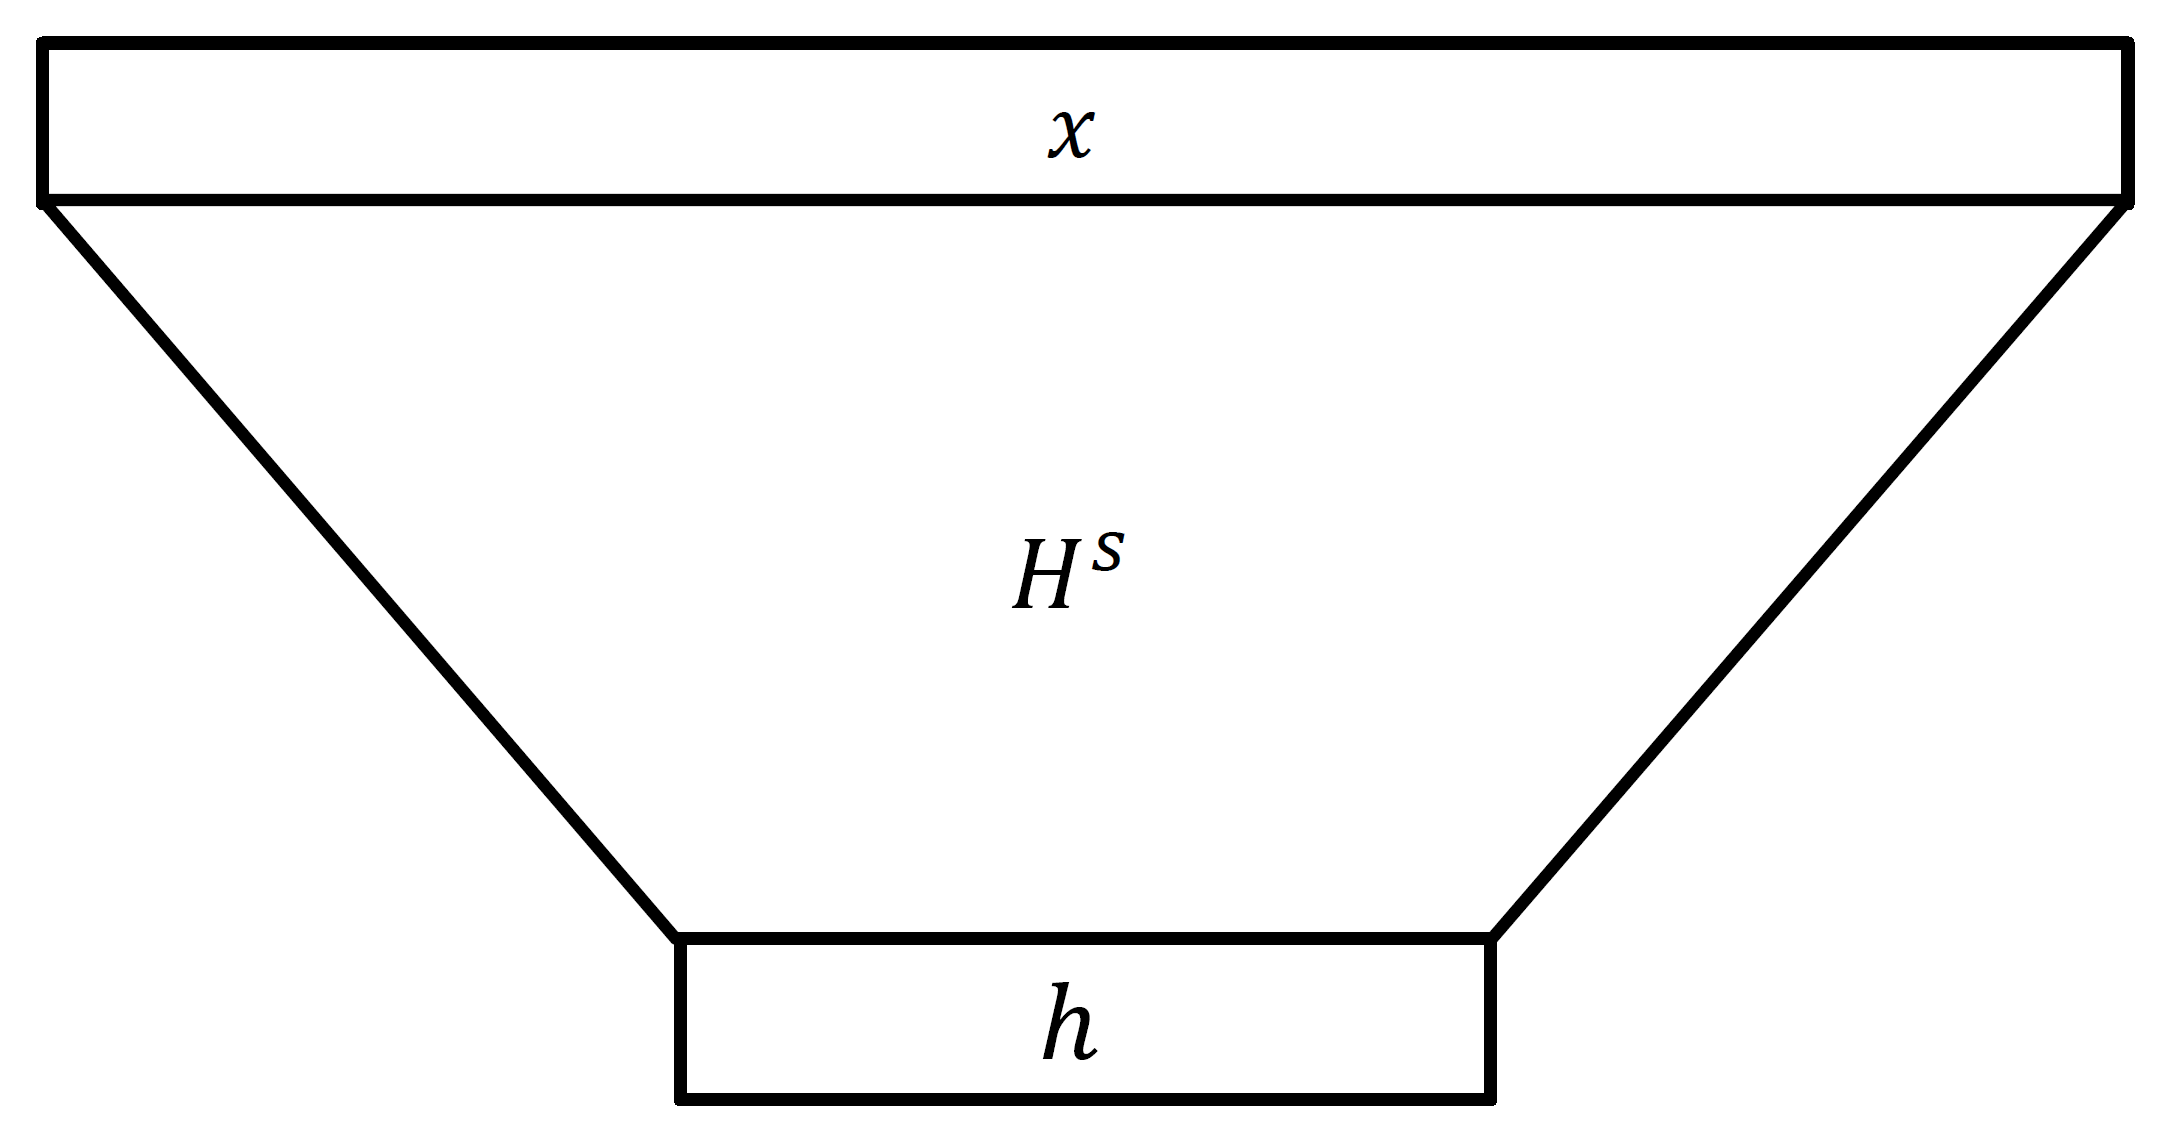
\includegraphics[width=120mm]{Graphics/Hash Functions/hf1.png}
	\end{center}
    \textbf{Remarks:}
    \begin{itemize}
        \item The output length $l=l(\lambda)$ only depends on $\lambda$
        \item If $H^S$ is only defined on inputs of length $l' > l$ we call $H$ a fixed-length hash function
        \item If we don't specify $Gen$ it just chooses uniformly random $s \leftarrow_{\$} \{0,1\}^{\lambda}$
    \end{itemize}
\end{definition}


\begin{definition}[Collision Resistance]
	Let $H: \{0,1\}^{l'} \to \{0,1\}^{l}$ with $l' > l$.\\
    A hash function $(Gen,H)$ is called collision-resistant, if for every PPT-bounded adversary $\mathcal{A}$ there exists a negligible function $v$ s.t. for all $\lambda \in \mathbb{N}$
    $$Pr[Hash-Col_{\mathcal{A}}(\lambda)=1] < v(\lambda)$$
   	\begin{center}
		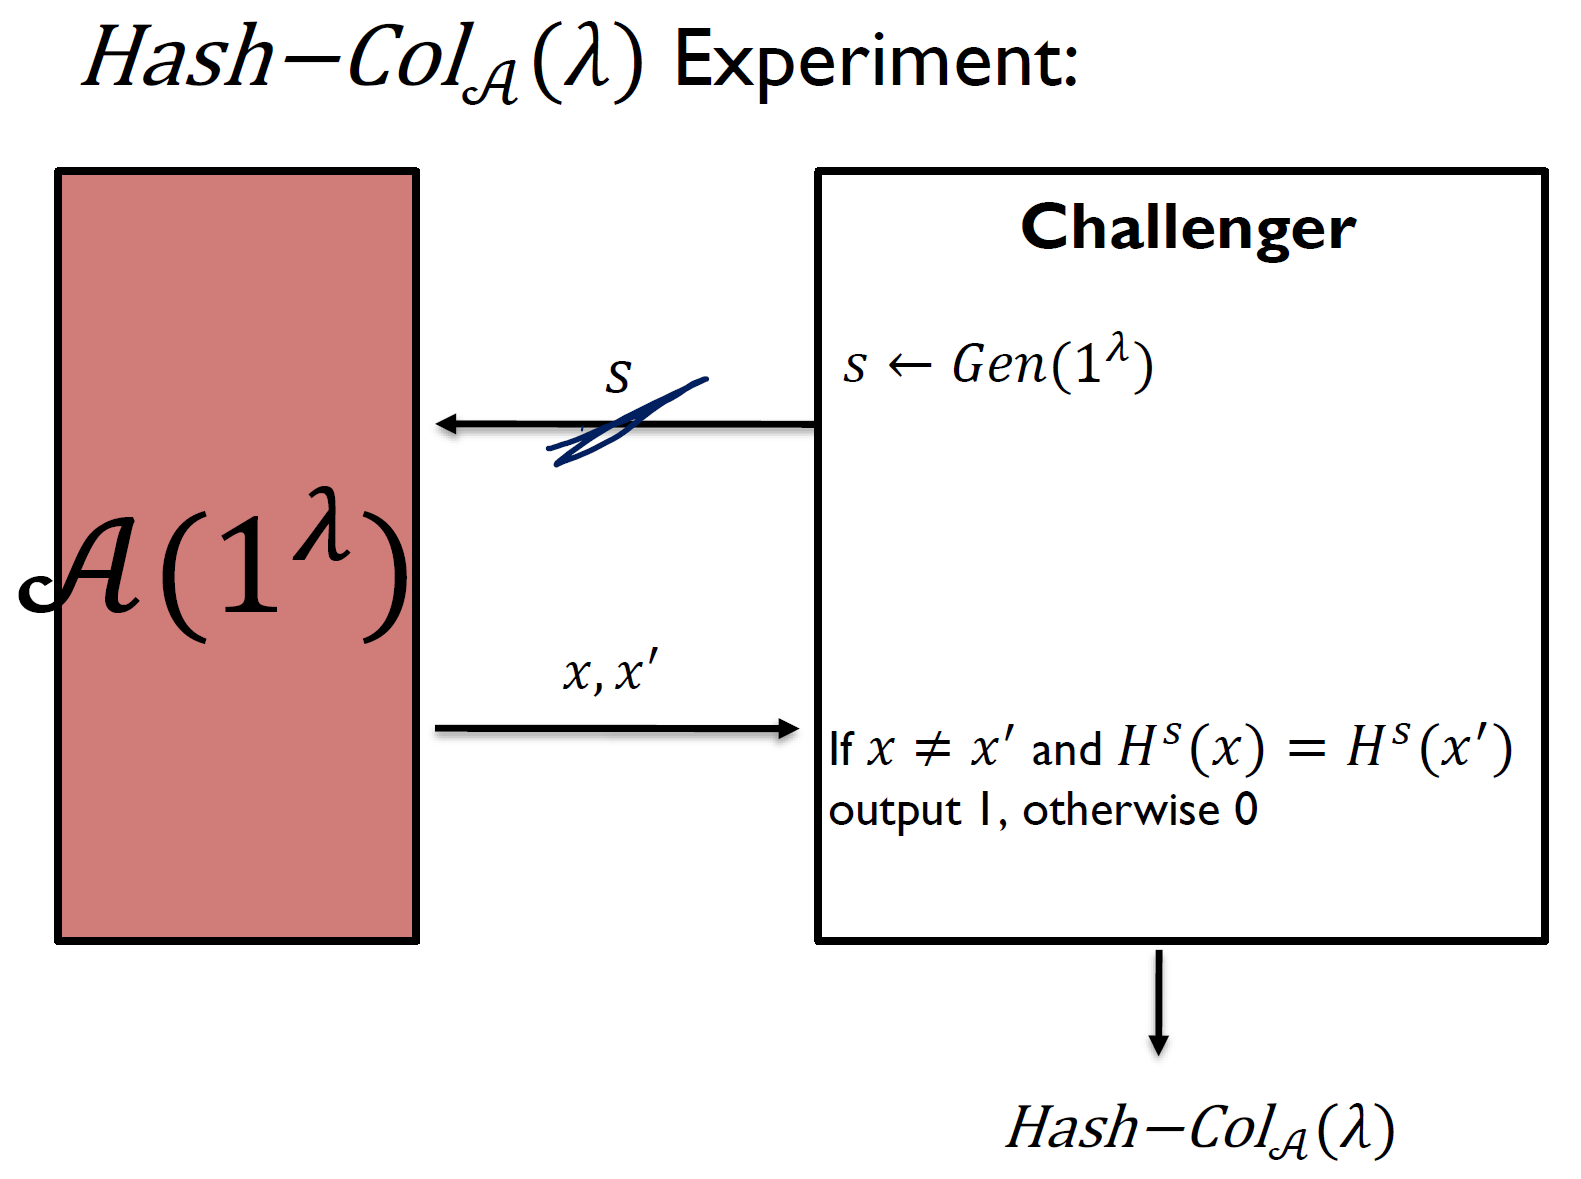
\includegraphics[width=120mm]{Graphics/Hash Functions/hf2.png}
	\end{center}
\end{definition}

	\subsection{Examples}
		\begin{itemize}
			\item Assume $H$ is a collision resistant hash function
			\item Is $H'$ given by $H'^S(x) = H^S(x || 0^{\lambda})$ also collision resistant?
			\begin{itemize}
				\item Yes!
				\item Idea: Collision $x,x'$ for $H'$ yields collision $x || o^{\lambda}$, $x' || 0^{\lambda}$ for $H$
			\end{itemize}
			\item Is $H''$ given by $H''^S(x_1...x_n) = H^S(x_1...x_{n-1})$ collision resistant?
			\begin{itemize}
				\item No!
				\item $0...00$ and $0...01$ hash to the same value
			\end{itemize}
		\end{itemize}


\section{Idealized Hash Functions}
	\begin{itemize}
	    \item Sometimes collision resistance isn’t enough…
	    \item Sometimes we need hash functions for which it is hard to find arbitrary correlations
	    \item E.g. for a fixed function $f$ it should be hard to find an input $x$ with $H^S(x)=f(x)$
	    \item How should an ideal hash function behave?
	    \item Like a random function!
	\end{itemize}


\section{The Random Oracle Model}
	\begin{itemize}
	    \item Random Oracle (RO): Uniformly random function $\mathcal{H}: \{0,1\}^l \to \{0,1\}^{\lambda}$ which can only be accessed via oracle access/blackbox access
	    \item Random oracle is uniform on positions it has not been queried on
	    \item Models a hash function whose code no-one knows
	    \item Rationale: The only way of learning something about a hash function which is modeled by RO is to evaluate it
	    \item To evaluate $\mathcal{H}$ adversary needs to provide input explicitly to random oracle
	    \item Idea: In security proofs reduction controls RO!
	\end{itemize}
   	\begin{center}
		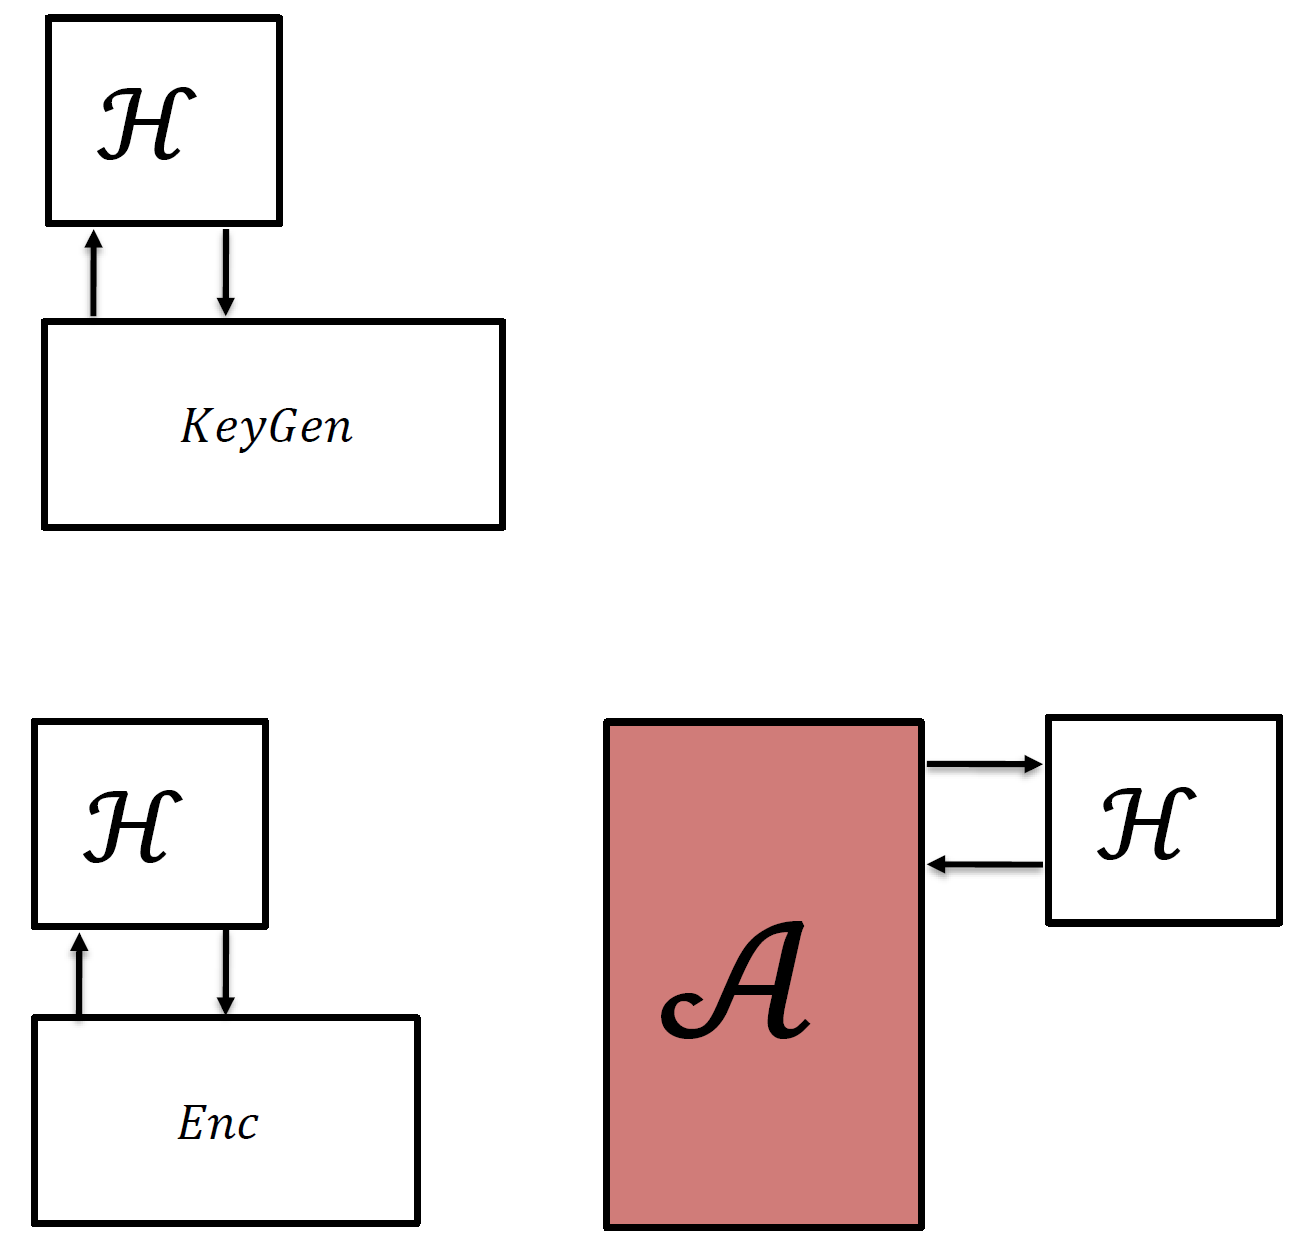
\includegraphics[width=110mm]{Graphics/Hash Functions/hf3.png}
	\end{center}
	\begin{itemize}
	    \item Obviously, real hash functions are not random oracles
	    \item E.g. real hash functions have small description (e.g. program)
	    \item Sometimes, we only know how to prove constructions secure if $\mathcal{H}$ is modeled as random oracle
	    \item Two step approach:
	    \begin{itemize}
	        \item Model hash function as a RO in the security proof
	        \item In the real world, instantiate with actual hash function
	    \end{itemize}
	    \item Better than no proof at all!
	    \item Proofs in RO model are heuristic
	    \item If a scheme is secure in the RO model, but insecure in real world, adversary must do something non trivial and interesting with hash function
	\end{itemize}

	\subsection{Examples}
		Random Oracle yields collision resistant hash function $H^S(x) = \mathcal{H}(s||x)$
	   	\begin{center}
			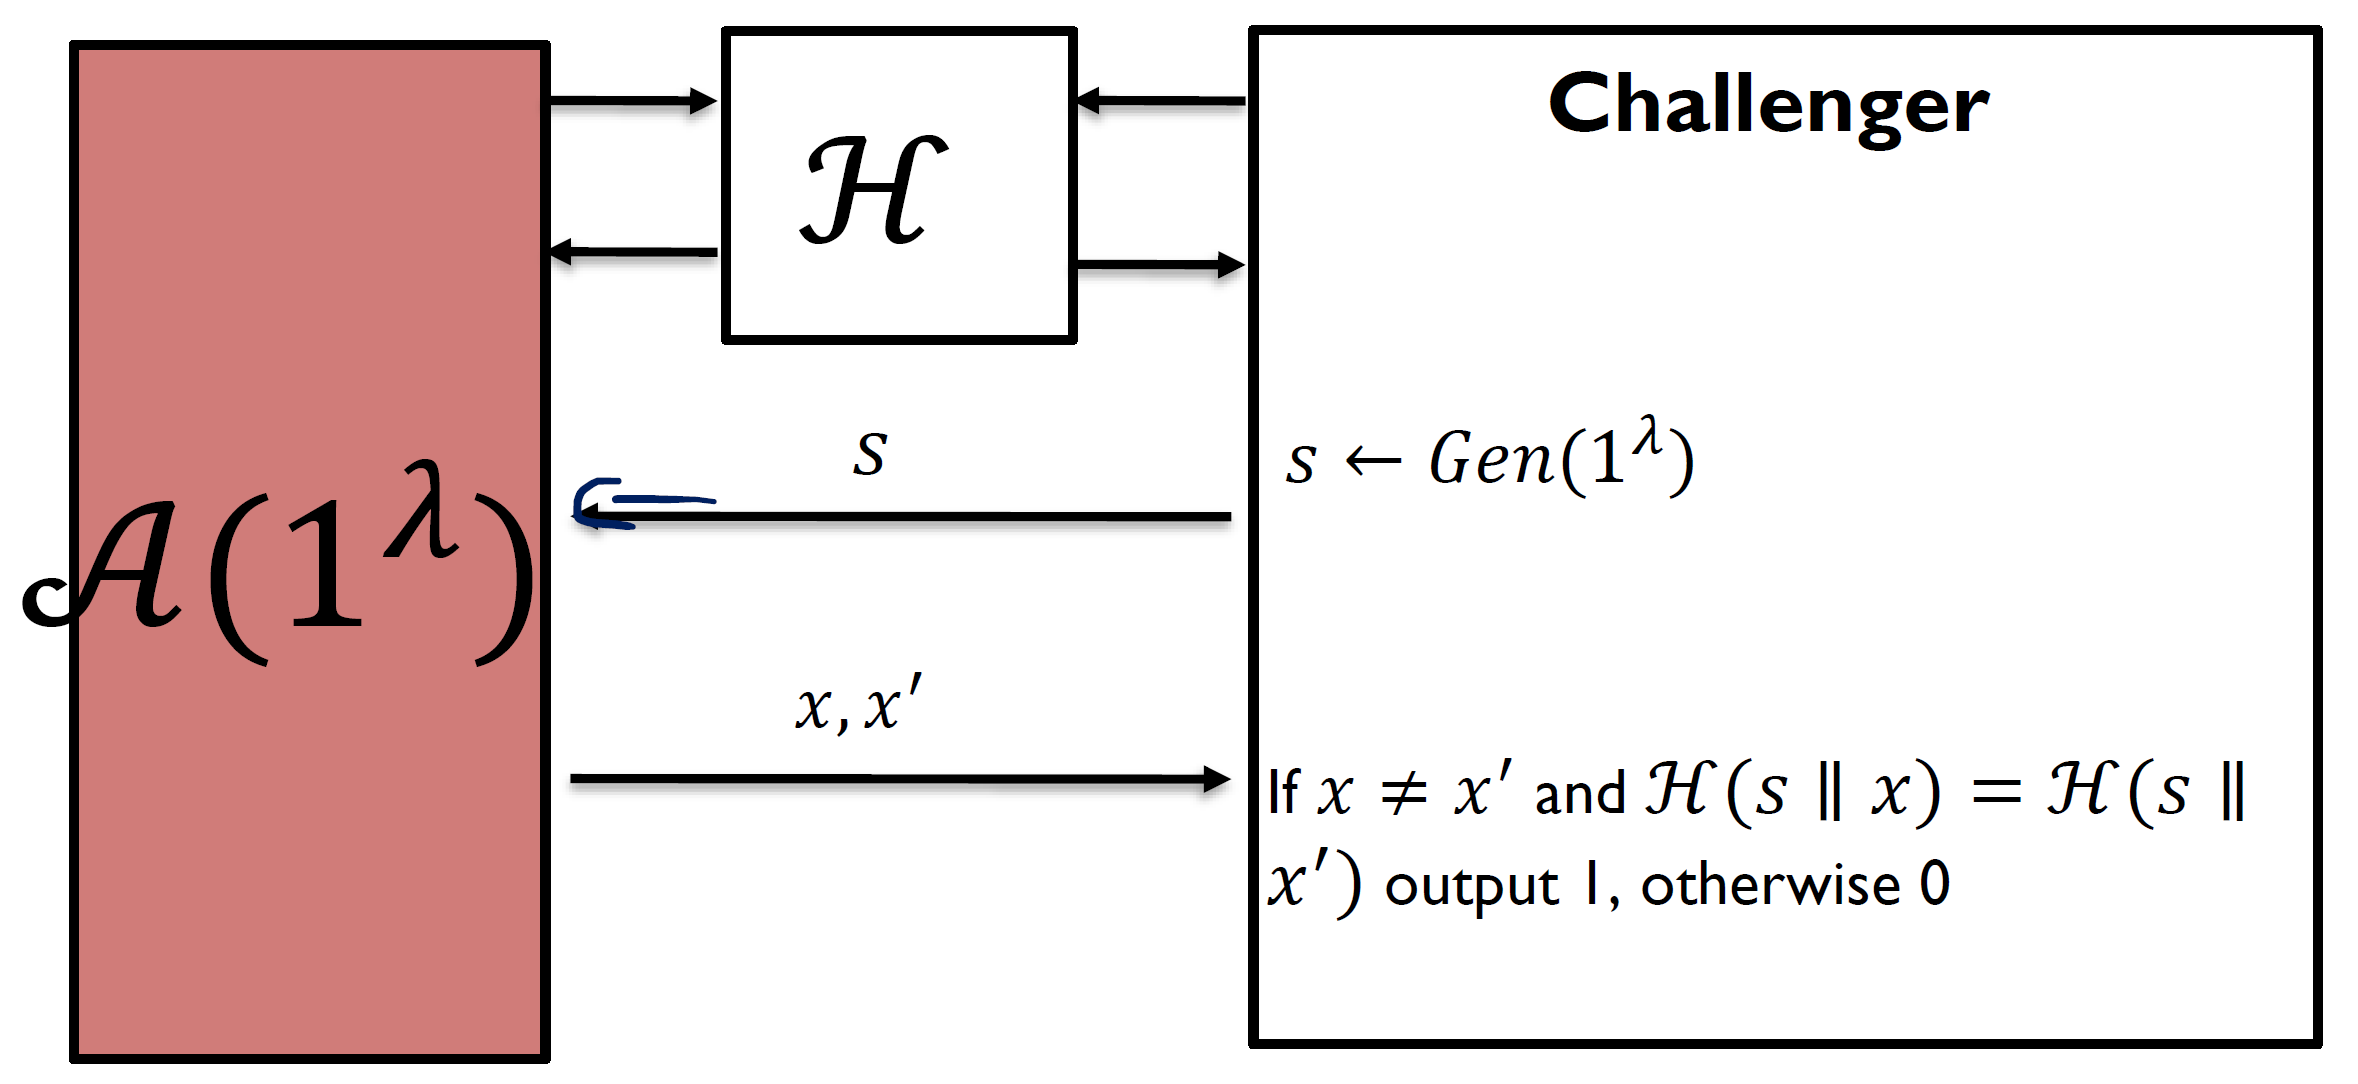
\includegraphics[width=140mm]{Graphics/Hash Functions/hf4.png}
		\end{center}
		\begin{proof}
			Assume $\mathcal{A}$ makes at most $q=poly(\lambda)$ queries $x_1,...,x_q$ to $\mathcal{H}$.\\
			$\mathcal{H}$ is uniformly random function, i.e. all function values are uniform and independent.\\
			Probability of single collision:
			$$Pr[\mathcal{H}(s||x_i) = \mathcal{H}(s||x_j)] = 2^{-\lambda}$$
			It follows that
			$$Pr[\exists i,j: \mathcal{H}(s||x_i) = \mathcal{H}(s||x_j)] \leq q^22^{-\lambda} = negl(\lambda) \text{(union bound)}$$
		\end{proof}

\section{Summary}
	\begin{itemize}
		\item Hash functions compress objects into short digests
		\item Digests are \textit{computationally} unique
		\item This is captured in the collision resistance property
		\item Random oracles model ideal hash functions with stronger properties
		\item RO model allows for easy proofs!
		\item Random oracle model is a heuristic: Proofs in the random oracle model don’t necessarily hold in the real world.
	\end{itemize}

\newpage
\begin{definition}[Security Definition]\ \\
    \textbf{The collision-finding experiment} $Hash-coll_{\mathcal{A},(Gen,H)}(n)$
    \begin{itemize}
        \item On input $s$, $\mathcal{A}$ outputs $x$ and $x'$.
        \item $Hash-coll_{\mathcal{A},??? (05-02,3)}(n) = 
        \begin{cases} 
        1 & x \neq x' $ and $ H^S(x)=H^S(x')\\
        0 & otherwise
        \end{cases}$
    \end{itemize}
    In the above experiment,
    \begin{itemize}
        \item $\mathcal{A}$ is polynomial time bounded;
        \item if no efficient adversary can find a collision except with negligible probability, then $(Gen;H)$ is collision resistant.
    \end{itemize}
    Some weaker security notions are also considered:
    \begin{itemize}
        \item second-preimage resistance: given $s$ and a random $x$, it is infeasible for a probabilistic polynomial-time adversary to find $x' \neq x$ such that $H^S(x') = H^S(x)$.
        \item preimage resistance: given $s$ and $a$ the hash $y = H^S(x_0)$ of a random $x_0$, it is infeasible for a probabilistic polynomial-time adversary to find $x$ such that $H^S(x) = y$.
    \end{itemize}
\end{definition}

\section{A word on Provable Security}
	\begin{itemize}
	    \item Hash functions in the real world are generally unkeyed and have a fixed output length.
	    \item Problematic from a theoretical standpoint.
	    \item Current hash functions are still collision resistant since no colliding pair is known, and would be computationally difficult to find.
	    \item A hash function with output length n is considered secure as long as:
	    \begin{itemize}
	        \item no known algorithm can find a colliding pair in time much smaller than $2^{n/2}$;
	        \item no known algorithm can find a preimage or second preimage in time much smaller than $2^n$.
	    \end{itemize}
	    \item Provable security for hash functions follows the same patterns as provable security for block ciphers.
	\end{itemize}

\section{The Merkle-Dåmgard construction}
   	\begin{center}
		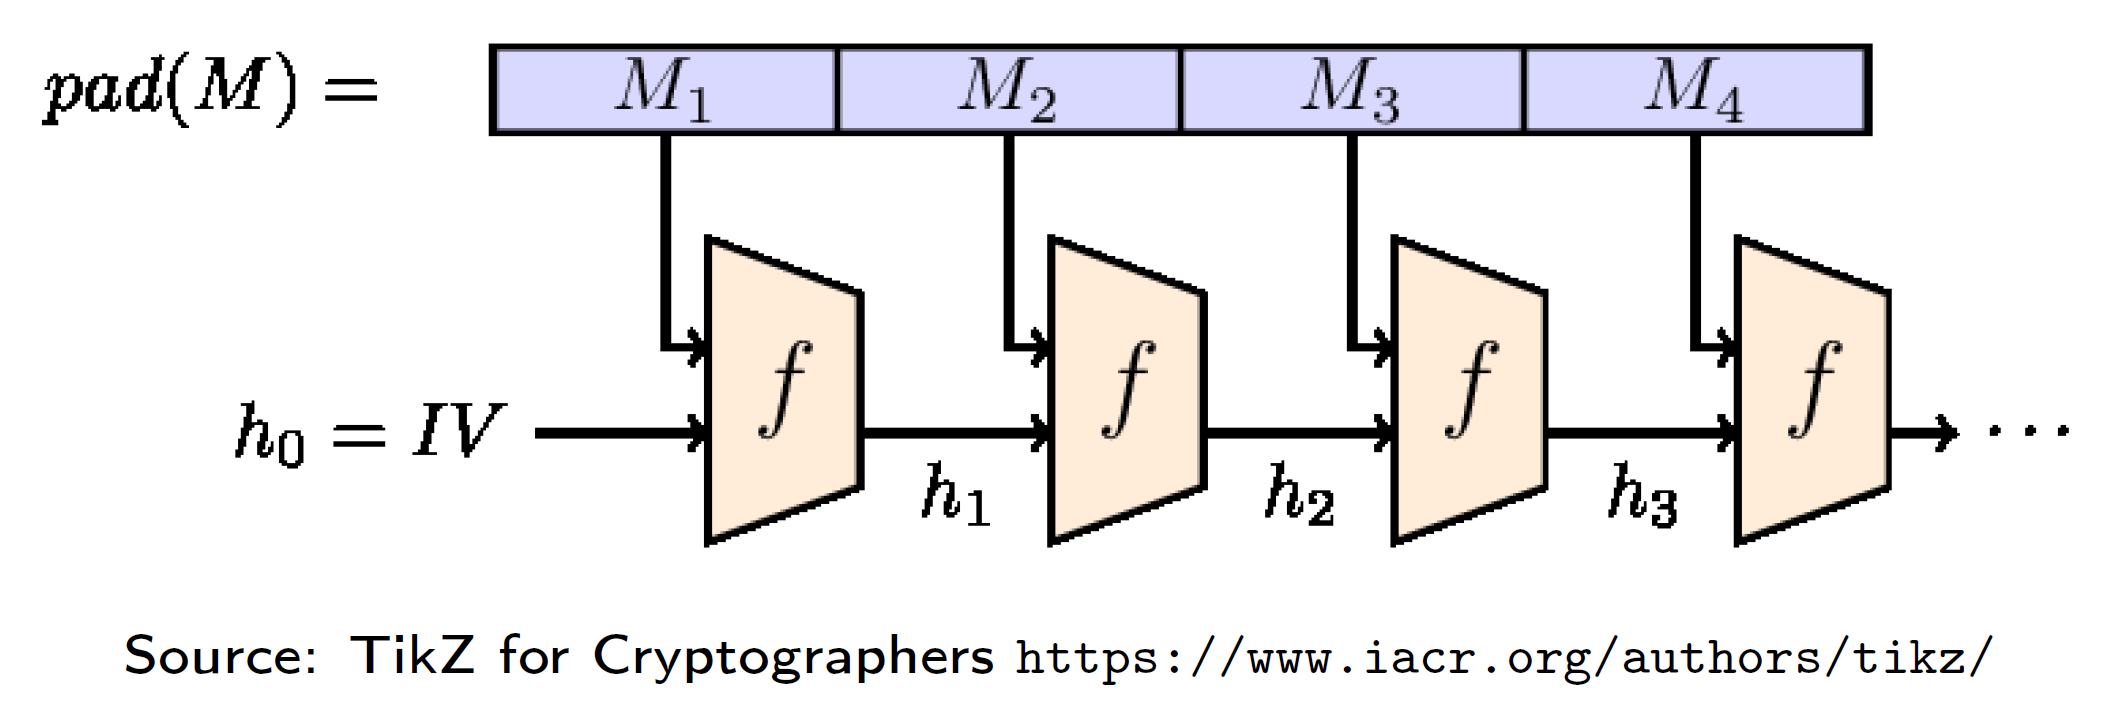
\includegraphics[width=140mm]{Graphics/Hash Functions/hf5.png}
	\end{center}
    \begin{itemize}
        \item $(Gen,f)$ is a fixed-length hash function for inputs of length $2n$ and outputs of length $n$.
        \item $(Gen,F)$ (as defined above) operates on strings of length $L < 2^n$.
        \item To compute $pad(M)$: pad the message $M$ with 0 until its length is a multiple of $n$, then add a final block that corresponds to $L$ encoded as an $n$-bit string.
        \item IV is called the \textit{initialization vector}, and is an arbitrary constant.
    \end{itemize}

	\begin{theorem}
	    If $(Gen,f)$ is collision resistant, so is $(Gen,F)$.
	\end{theorem}
	\begin{proof}
		Proofsketch:
		\begin{itemize}
			\item Assume you know $x \neq x'$ such that
			\begin{itemize}
				\item $F^S(x) = F^S(x')$;
				\item $x$ and $x'$ are of respective length $L$ and $L'$ (in bits);
				\item $M = pad(x)$ and $M' = pad(x')$ are of length $B$ and $B'$ (in blocks). 
			\end{itemize}
			\item Case $L \neq L'$: one has $f^S(h_B||L) = f^S(h'_{B'}||L')$, which gives a collision under $f^S$.
			\item Case $L=L'$:
			\begin{itemize}
				\item let $l_i = h_{i-1}||M_i$, $l'_i = h'_{i-1}||M'_i$, and $I_{B+2} = F^S(x) = F^S(x') = I'_{B+2}$;
				\item let $i_0$ be the largest index for which $l_{i_0} \neq l'_{i_0}$.
				Necessarily, $i_0 \leq B+1$.
				\item by maximality of $i_0$, $l_{i_0} \neq l'_{i_0 +1}$, thus $f^S(l_{i_0}) = f^S(l'_{i_0})$, and $l_{i_0} \neq l'_{i_0}$,
				which gives a collision under $f^S$.
			\end{itemize}
		\end{itemize}
	\end{proof}
	
	\textbf{Is the previous theorem sufficient in practice?}
	\begin{itemize}
		\item Second preimages of (very) long messages can be found much faster than exhaustive search (but it still requires finding collisions for the hash function).
		\item Length extension: given the hash of an unknown message $x$, it is trivial to compute the hash of $pad(x)||y$ for any message $y$.
		\item Length extension attacks have actually been used in practice: one has to be careful when using a hash function based on the Merkle-Dåmgard construction in practice.
	\end{itemize}

\section{The Design of Compression Functions}
	General structure of the compression functions that we are going to deal with in the examples:
	\begin{itemize}
	    \item The function operates over $w$-bit words.
	    \item Its input is divided in two parts: a state, which stores the output of the previous call to the compression function, and a block of $n_c$ words of padded data.
	    \item Compression functions are generally iterative: a simple round is repeated $r$ times.
	    \item A linear function extends the $n_c$ words of data into $r$ words of extended data.
	    \item At each round, the state is updated with a nonlinear function, and a round constant and a word of extended data are absorbed in the state.
	\end{itemize}


\section{Sponge Functions}
   	\begin{center}
		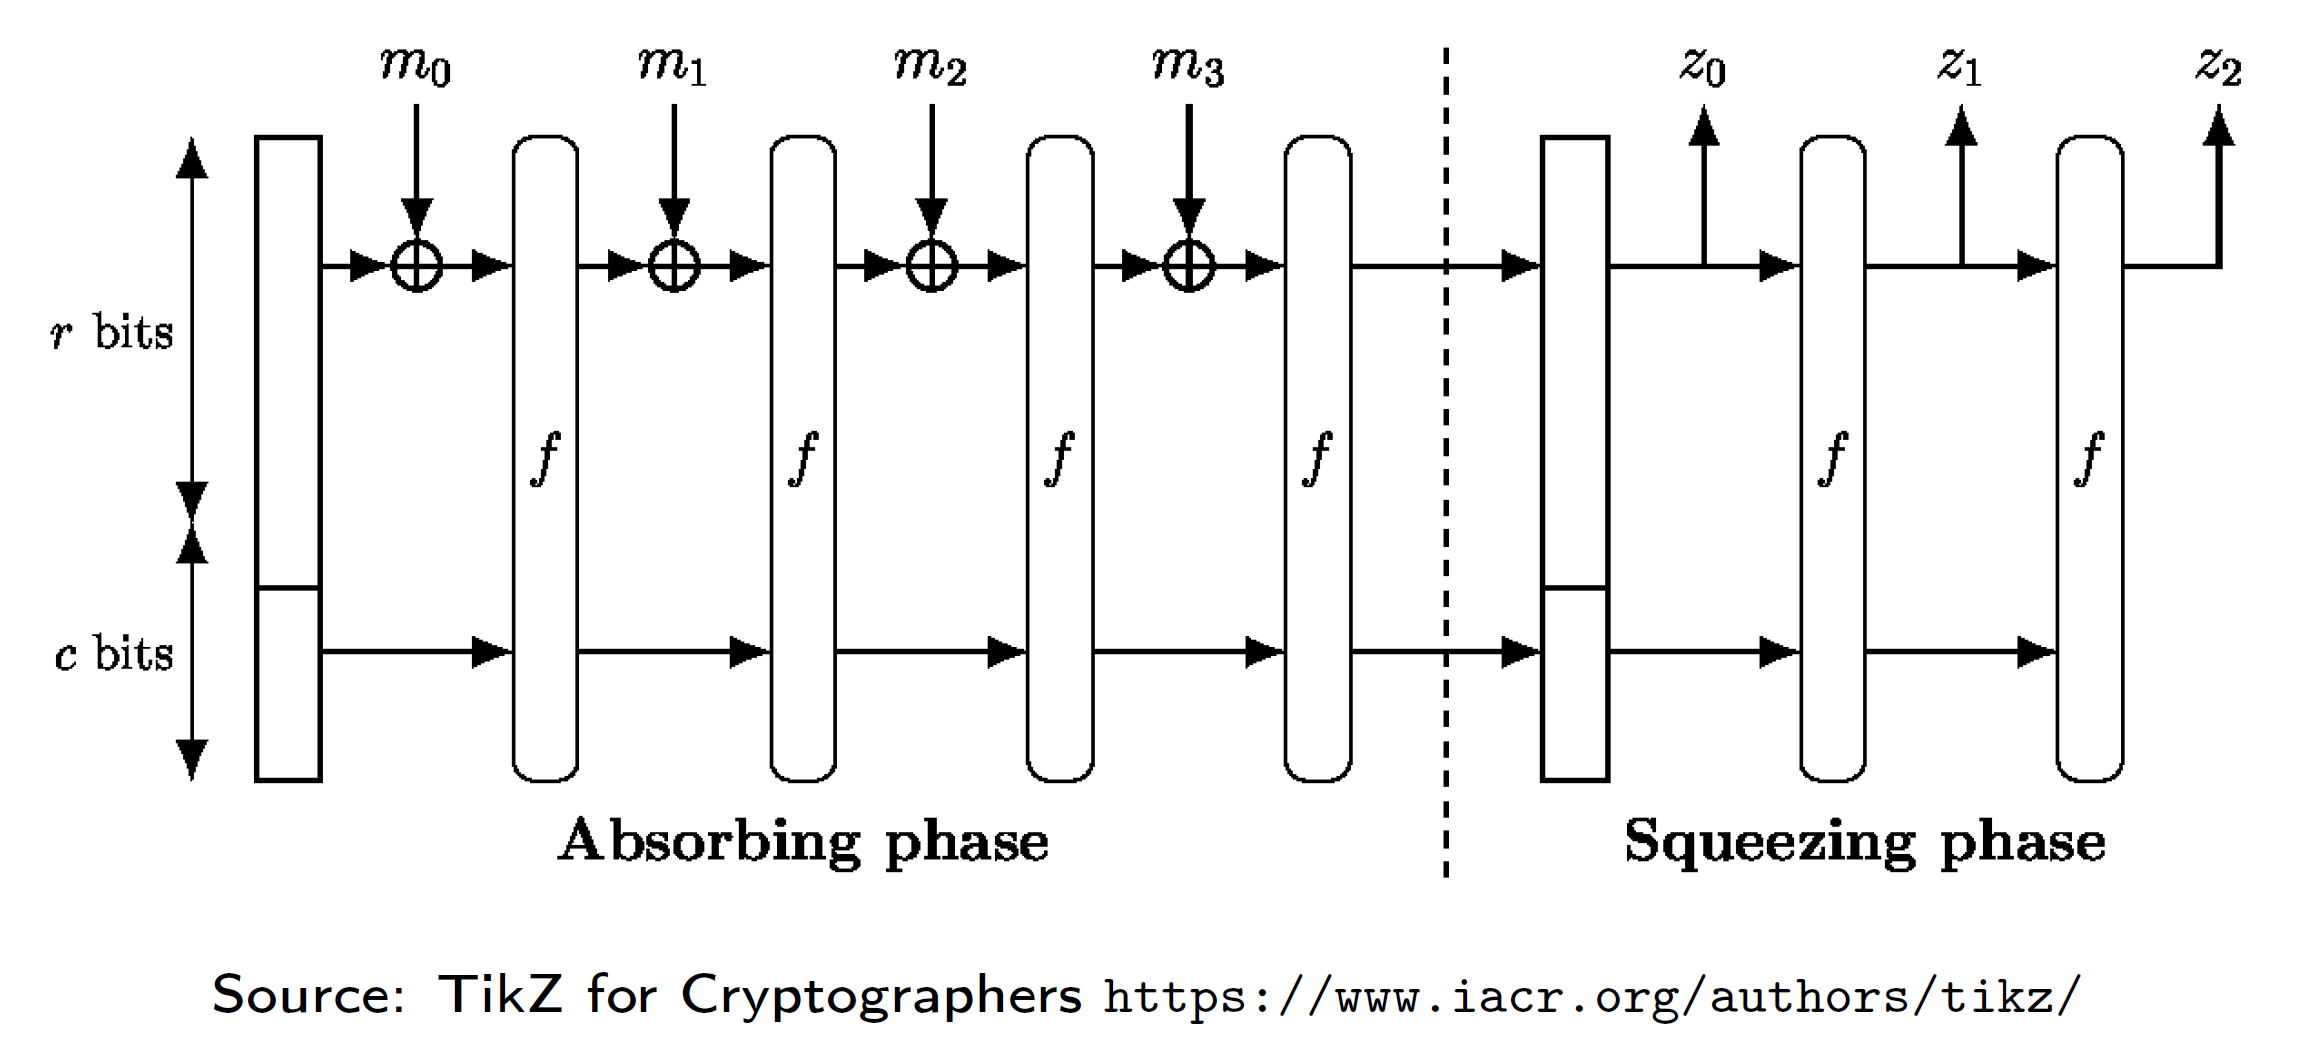
\includegraphics[width=140mm]{Graphics/Hash Functions/hf6.png}
	\end{center}
    \begin{itemize}
        \item Generic structure to build a hash function from a public and unkeyed function $f$.
        \item $f$ is usually a permutation.
        \item The $b$-bit function is repeatedly applied to a state consisting in:
        \begin{itemize}
            \item a $r$-bit outer state, where $r$ is called the rate;
            \item a $c$-bit inner state, where $c=b-r$ s called the capacity.
        \end{itemize}
        \item Padding of a message can be done by appending a single bit 1, followed by bits 0 until the length of the result is a multiple of $r$.
    \end{itemize}

\section{A word on Provable Security}
	How to justify the soundness of the sponge construction?
	\begin{itemize}
	    \item The function $f$ is fixed and public. To study the structure, we model it as a uniformly random function (or permutation). The resulting construction is called a random sponge.
	    \item How close is the random sponge from a random oracle?
	\end{itemize}

	\begin{definition}
	    Let $D$ be a probabilistic algorithm that deals at most $q$ oracle queries. Its distinguishing advantage is defined as
	    $$\mathcal{A}_{Sponge}^{dist}(D) \coloneq \vert Pr[D^{Sponge[f](\cdot)}=1]-Pr[D^{H(\cdot)}=1] \vert,$$
	    where the first probability is taken over the uniformly random draw of $f: \{0,1\}^b \to \{0,1\}^b$ and the second one over the uniformly random draw of the function $H$.
	\end{definition}

	\begin{itemize}
	    \item However, for a concrete hash function, $f$ is public!
	    \item An adversary has access to any intermediate value.
	    \item Hence, we have to give access to $f$ when the adversary is interacting with $Sponge[f]$.
	    \item In the random function case, a simulator is defined. It is a probabilistic polynomial time algorithm with access to the random oracle, 
	    whose goal is mimic the internal function of a random sponge.
	\end{itemize}

	\begin{definition}
	    Let $D$ be a probabilistic algorithm that deals at most $q$ oracle queries. Its differentiating advantage is defined as
	    $$\mathcal{A}_{Sponge}^{diff,S}(D) \coloneq \vert Pr[D^{Sponge[f](\cdot),f(\cdot)}=1]-Pr[D^{H(\cdot),S[H](\cdot)}=1] \vert,$$
	    where the first probability is taken over the uniformly random draw of $f: \{0,1\}^b \to \{0,1\}^b$ and the second one over the uniformly random draw of the function $H$.
	\end{definition}
	
	\begin{theorem}\label{thPS}
		There exists a simulator $S$ such that, for every a probabilistic algorithm $D$ whose queries require at most $q < 2^c$ calls to $f$, one has
		$$\mathcal{A}_{Sponge}^{diff,S}(d) \leq 1 - \prod\limits_{i=1}^q (1 - \frac{i}{2^c}) \lessapprox \frac{q(q+1)}{2^{c+1}}$$
	\end{theorem}
	
	Interpretation of theorem \ref{thPS}:
	\begin{itemize}
	    \item It does not provide actual security guaranties for any concrete hash functions.
	    \item But it does justify the soundness of the structure.
	    \item It also provides a lower bound on the capacity: $c \geq 2n$, where $n$ is the output length.
	\end{itemize}

\section{Examples}
	\subsection{Example 1: The MD5 Hash Function}
		\begin{itemize}
			\item Designed by Rivest in 1991.
			\item Produces a 128-bit hash.
			\item Built using the The Merkle-Dåmgard construction.
			\item Considered obsolete: collisions can be found in $2^{18}$ operations.
			\item Compression function takes as input the concatenation of the previous 128-bit output and the next 512-bit of padded message.
		\end{itemize}
	   	\begin{center}
			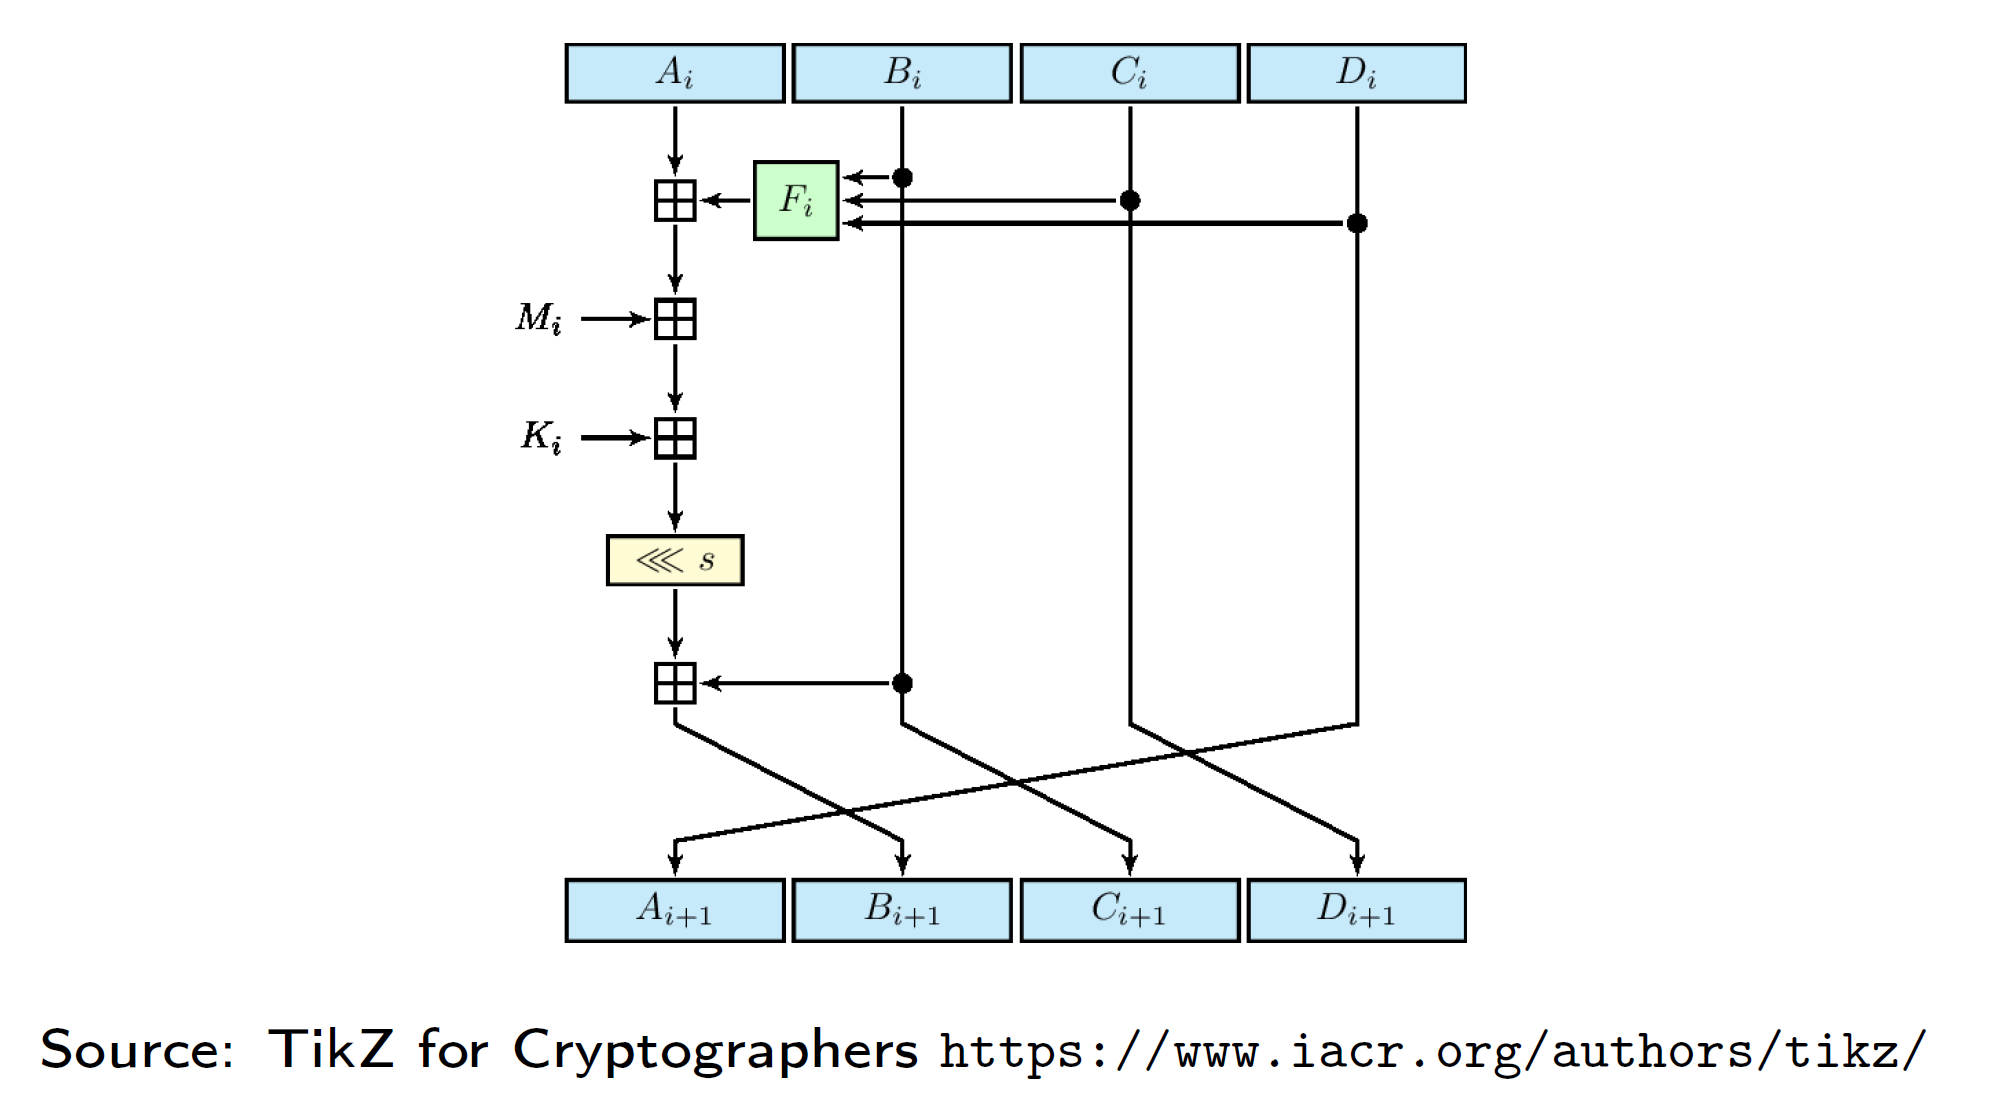
\includegraphics[width=140mm]{Graphics/Hash Functions/hf7.png}
		\end{center}
		\begin{itemize}
			\item MD5 compression function consists in 4 rounds of 16 MD5 operations.
			\item $A_i$, $B_i$, $C_i$, $D_i$ are the four 32-bit words that form the state.
			\item $F_i$ is a non-linear function that uses bitwise NOT, XOR, AND and OR operations. It depends on the round number.
			\item The "square with cross"-symbol denotes addition modulo $2^{32}$.
			\item At each operation, a 32-bit word $M_i$ of data and a constant $K_i$ are absorbed in the state.
		\end{itemize}
	
	\subsection{Example 2: The SHA-1 Hash Function}
		\begin{itemize}
			\item Designed by the United States National Security Agency in 1995.
			\item Closely related to the MD5 hash function.
			\item Considered obsolete: collisions are known, and can be found in around $2^{63.1}$ SHA1 evaluations.
			\item Produces a 160-bit hash.
			\item Compression function takes as input the concatenation of the previous 160-bit output and the next 512-bit of padded message.
		\end{itemize}
	   	\begin{center}
			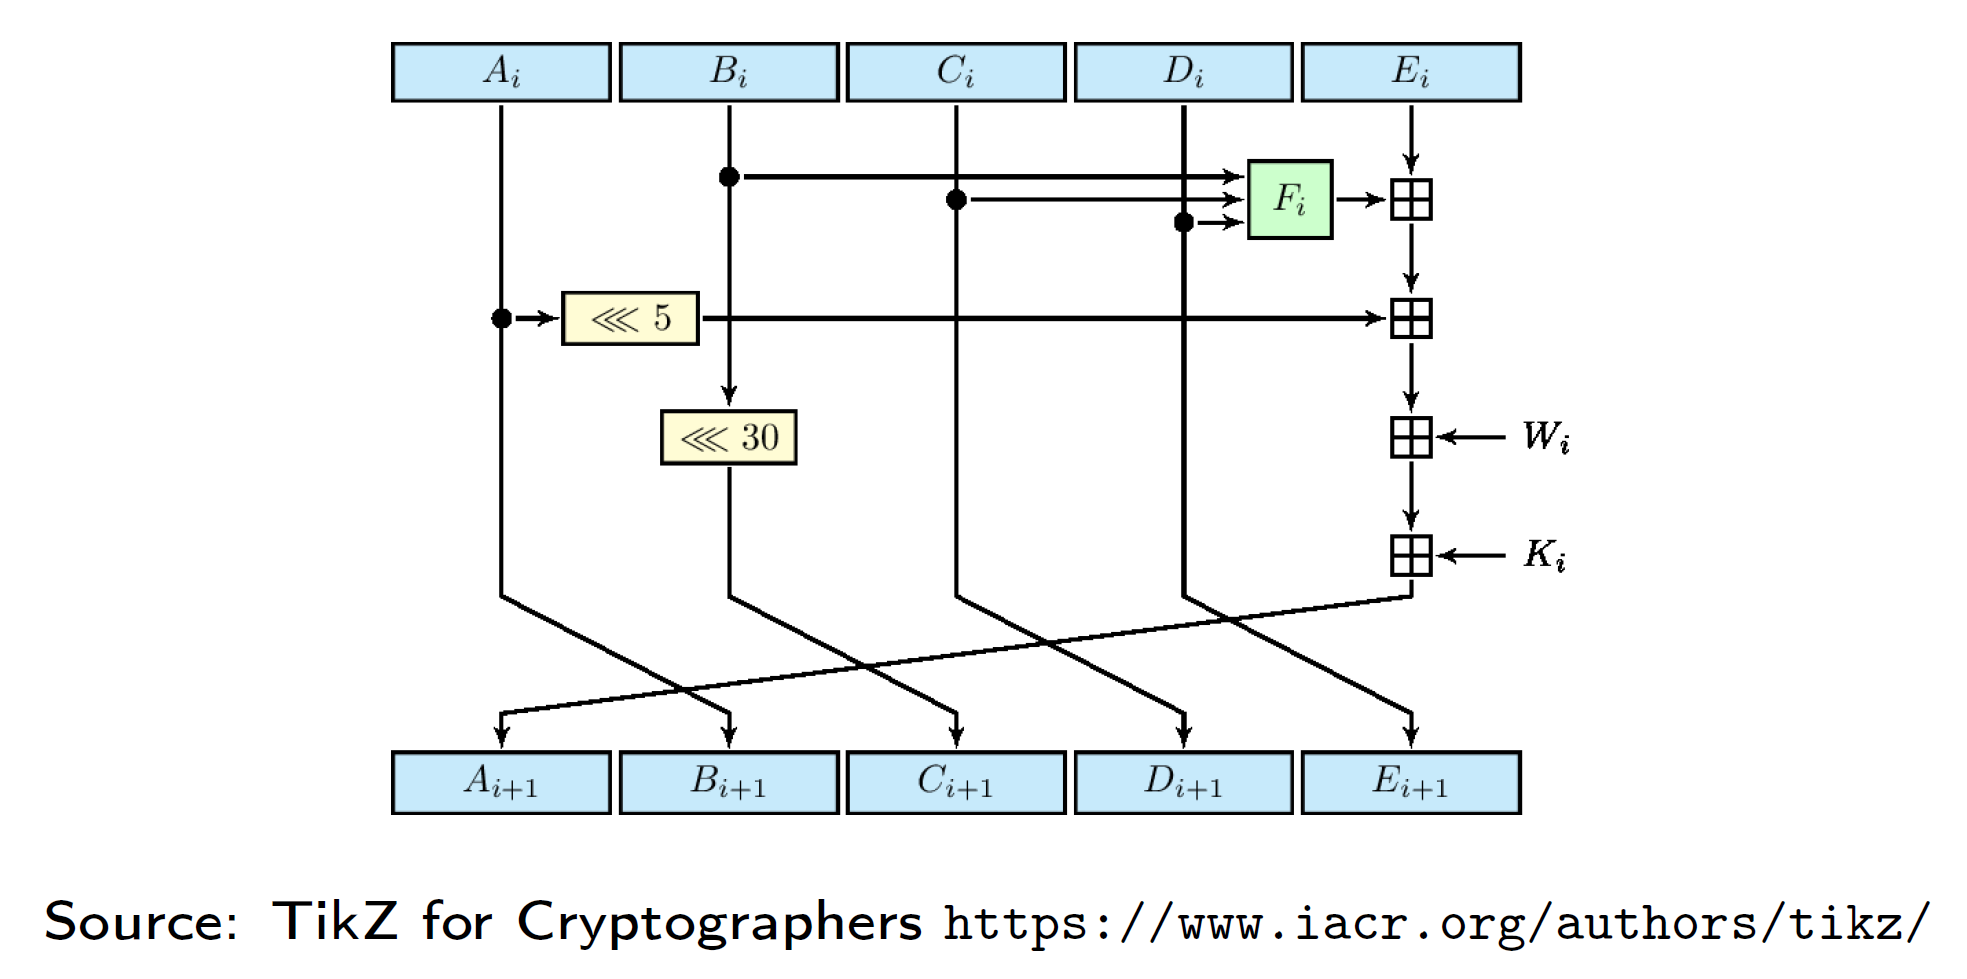
\includegraphics[width=140mm]{Graphics/Hash Functions/hf8.png}
		\end{center}
		\begin{itemize}
			\item SHA-1 compression function consists in 80 rounds. The new 512 bits of data are linearly extended to 80 32-bit words $(W_i)_{1 \leq i \leq 80}$.
			\item $A_i$, $B_i$, $C_i$, $D_i$ are the five 32-bit words that form the state.
			\item $F_i$ is a non-linear function that uses bitwise NOT, XOR, AND and OR operations. It depends on the round number.
			\item At round $i$, a 32-bit word $W_i$ of data and a constant $K_i$ are absorbed in the state.
		\end{itemize}
	
	\subsection{Example 3: The SHA-2 family of Hash Functions}
		\begin{itemize}
			\item Designed by the United States National Security Agency in 2001.
			\item Evolution of the SHA-1 hash function.
			\item Consists in a family of 6 hash functions with output lengths of 224, 256, 384 or 512 bits: SHA-224, SHA-256, SHA-384, SHA-512, SHA-512/224, SHA-512/256.
			\item Actually, only 2 hash functions: SHA-256 and SHA-512, the rest are truncated versions with different initial values.
			\item Both use similar compression functions. They differ by the size of the words on which they operate (32 bits and 64 bits), the number of rounds (64 and 80), and the round constants.
			\item Still considered secure nowadays.
		\end{itemize}
	   	\begin{center}
			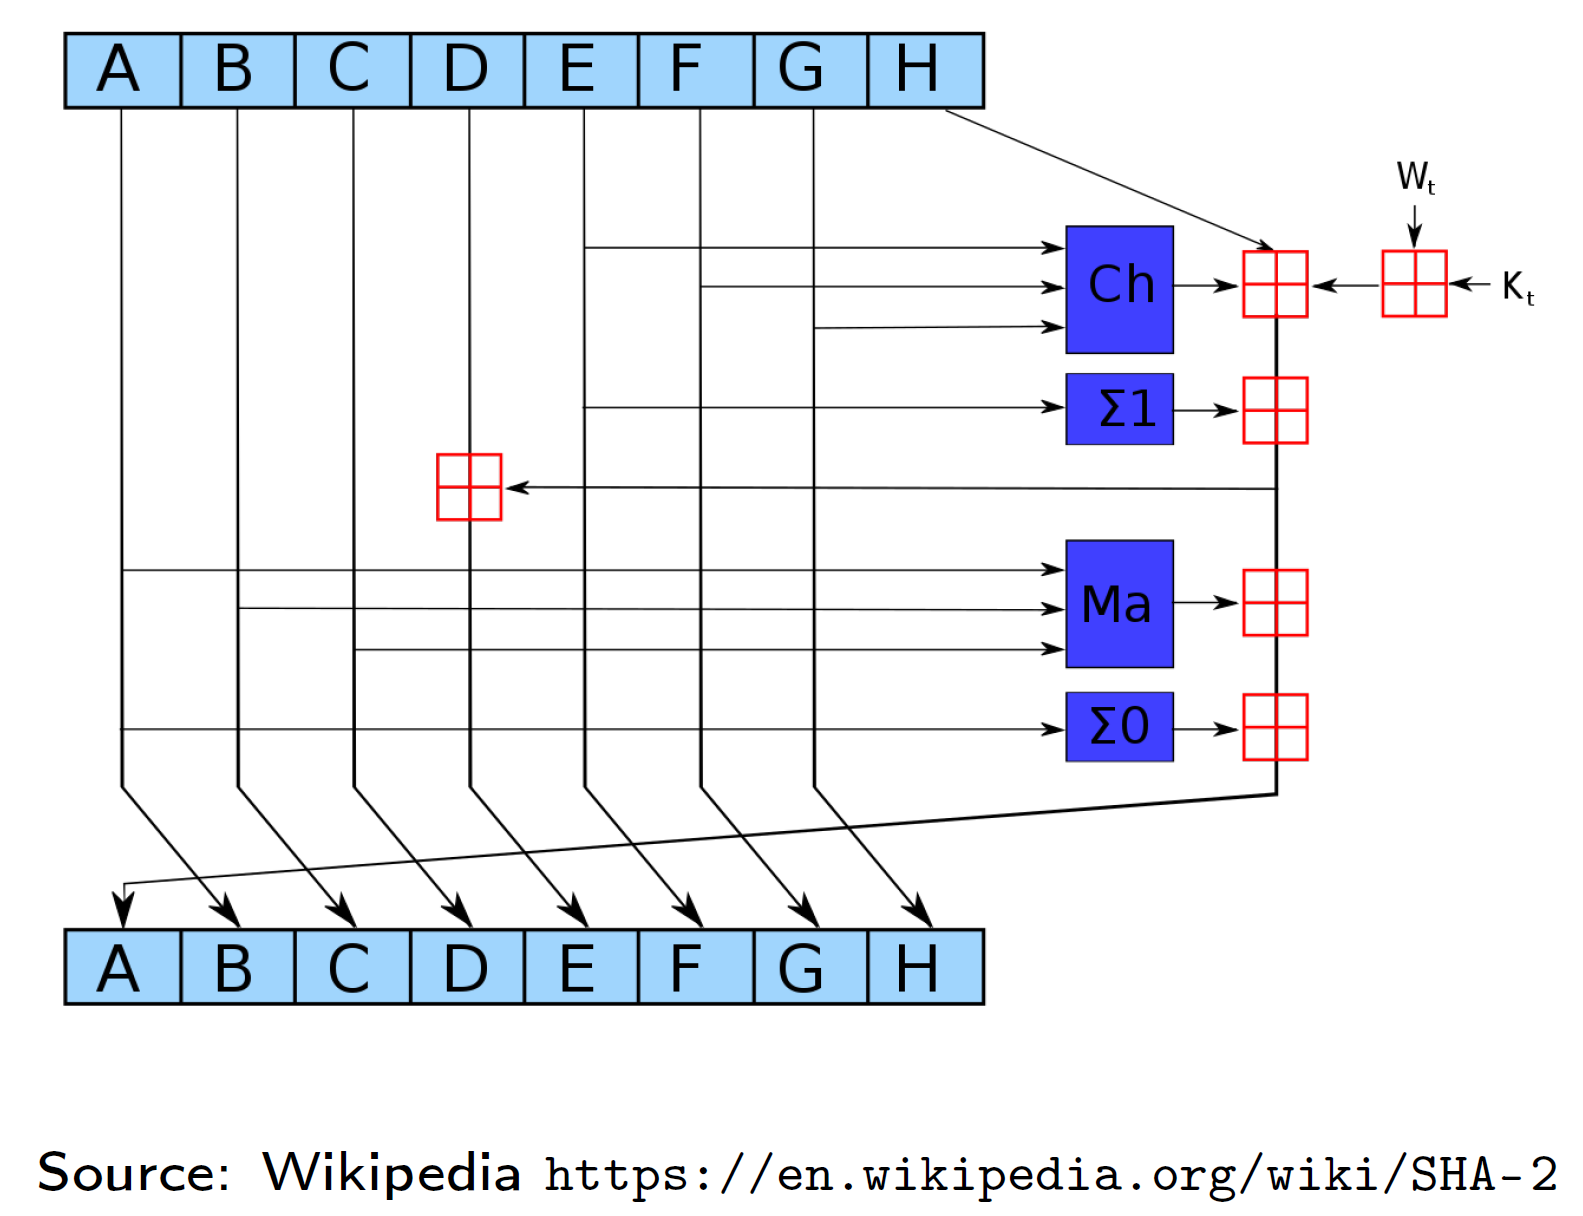
\includegraphics[width=140mm]{Graphics/Hash Functions/hf9.png}
		\end{center}
		\begin{itemize}
			\item $A,...,H$ are the 8 words of the state (block length is still 16 words).
			\item $Ch(E,F,G) = (E \wedge F) \oplus (\neg E \wedge G)$
			\item $Ma(A,B,C) = (A \wedge B) \oplus (A \wedge C) \oplus (B \wedge C)$
			\item $\sum_0(A) = (A \ggg 2) \oplus (A \ggg 13) \oplus (A \ggg 22)$
			\item $\sum_1(E) = (E \ggg 6) \oplus (E \ggg 11) \oplus (E \ggg 25)$
			\item Bitwise rotation constants differ between both round functions (here SHA-256).
		\end{itemize}
	
	\subsection{Example 4: The SHA-3 family of Hash Functions}
		\begin{itemize}
			\item United States National Institute of Standards and Technology (NIST) standard adopted in 2015 after an open competition.
			\item Based on the winner of the competition: Keccak (designed by Guido Bertoni, Joan Daemen, Michaël Peeters, and Gilles Van Assche).
			\item Based on the sponge construction with the $10*1$ padding. 
			All instances use the same Keccak-f[1600] permutation.
			\item Actually a set of 4 algorithms:
			\begin{center}
				\begin{tabular}[h]{lllll}
					Instance & Output size & Rate & Capacity & Definition\\
					SHA3-224(M) & 224 & 1152 & 448 & Keccak[448](M || 01, 224)\\
					SHA3-256(M) & 256 & 1088 & 512 & Keccak[512](M || 01, 256)\\
					SHA3-384(M) & 384 & 832 & 768 & Keccak[768](M || 01, 384)\\
					SHA3-512(M) & 512 & 576 & 1024 & Keccak[1024](M || 01, 512)
				\end{tabular}
			\end{center}
			\item Keccak[c]$(\cdot, d)$ denote the Keccak sponge, with capacity $c$, and output size $d$.
			\item Current standard, considered highly secure.
		\end{itemize}
	   	\begin{center}
			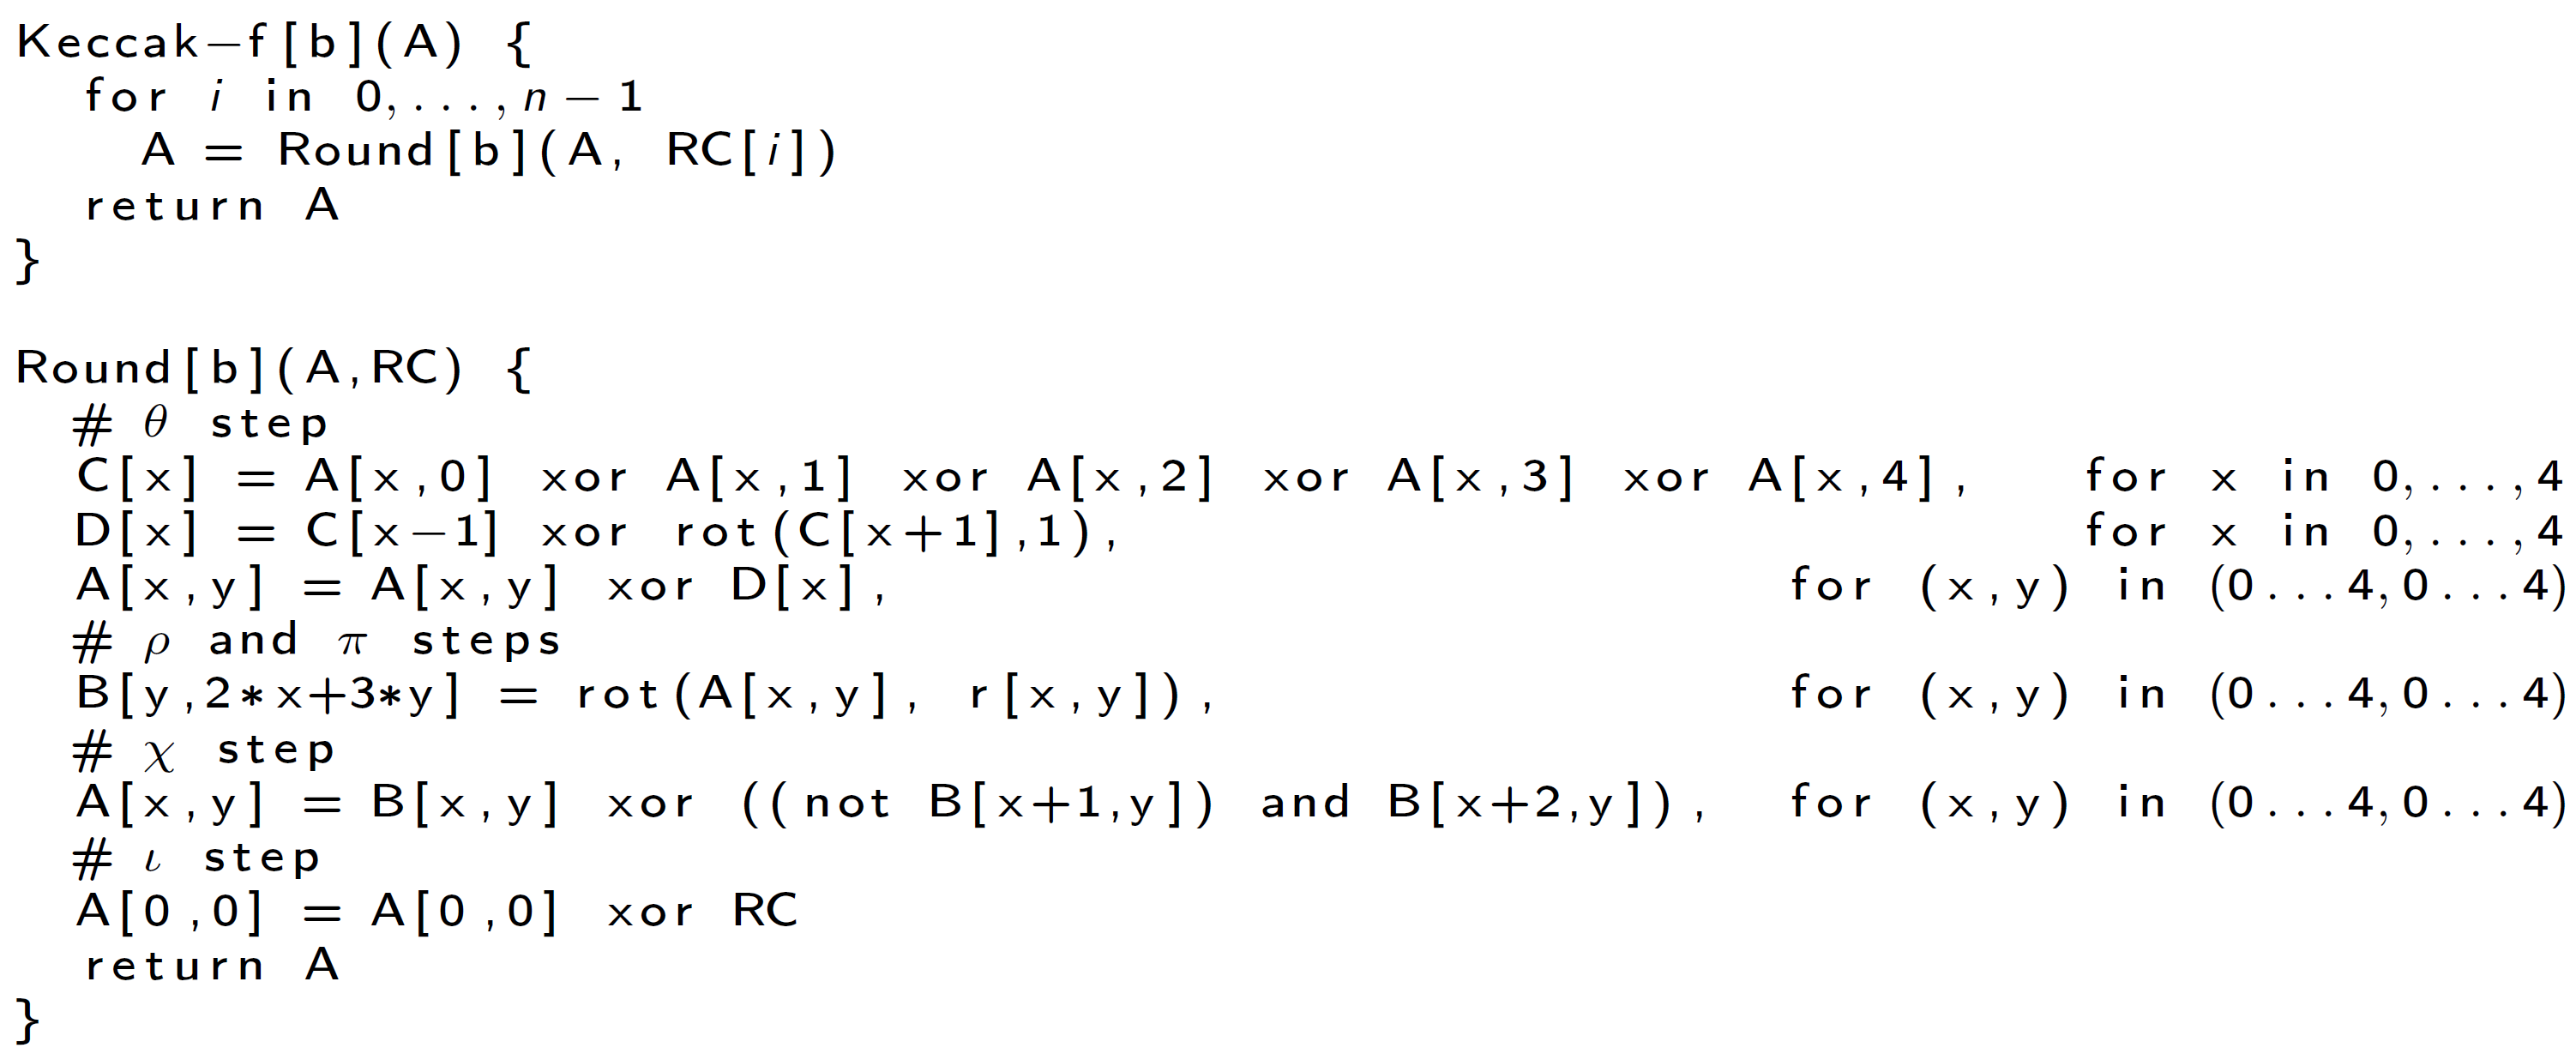
\includegraphics[width=140mm]{Graphics/Hash Functions/hf9.5.png}
		\end{center}
		\begin{itemize}
			\item 7 different variants for $b \in \{25, 50, 100, 200, 400, 800, 1600\}$
			\item The state consists in 25 words of size $w = \frac{b}{25}$.
			\item The number $n$ of rounds is computed as $n = 12 + 2l$ where $w = 2^l$.
		\end{itemize}

		\subsubsection{The Keccak-f[200] Permutation}
			\begin{center}
				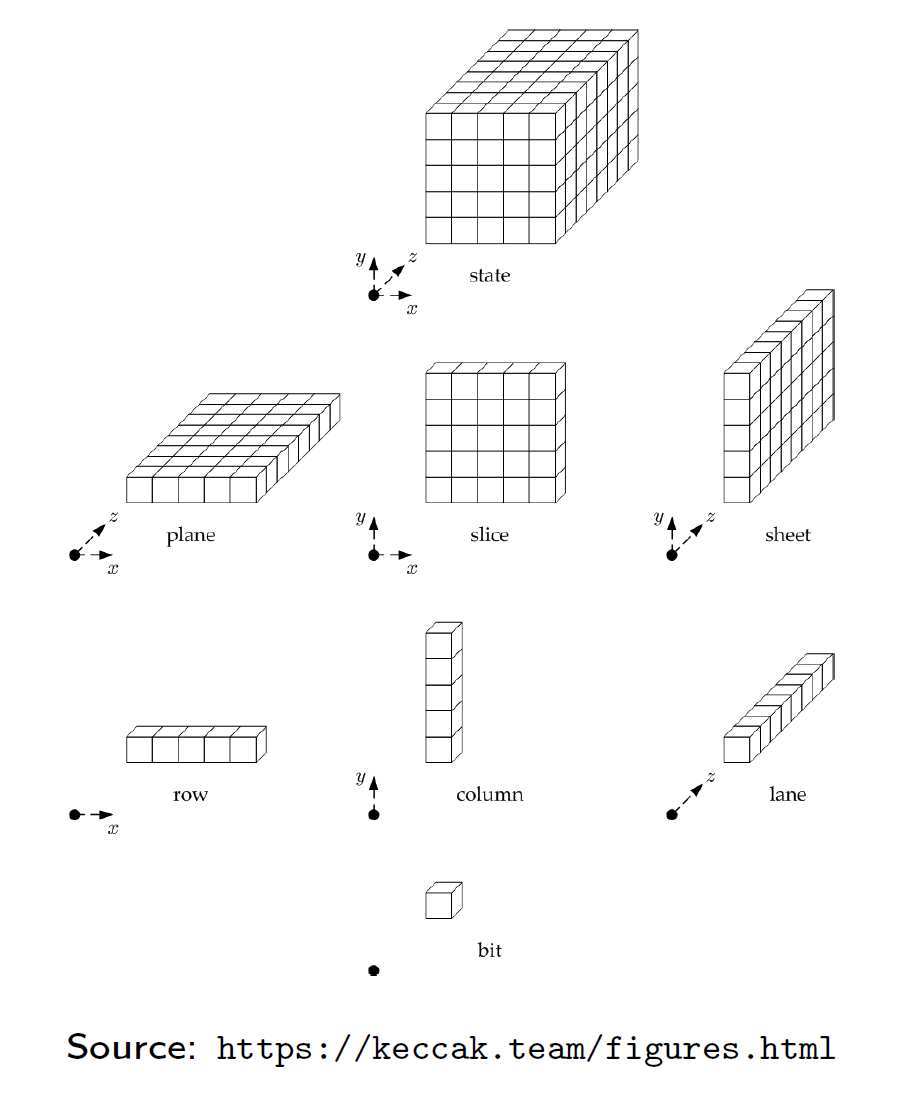
\includegraphics[width=120mm]{Graphics/Hash Functions/hf10.png}
			\end{center}
		   	\begin{center}
				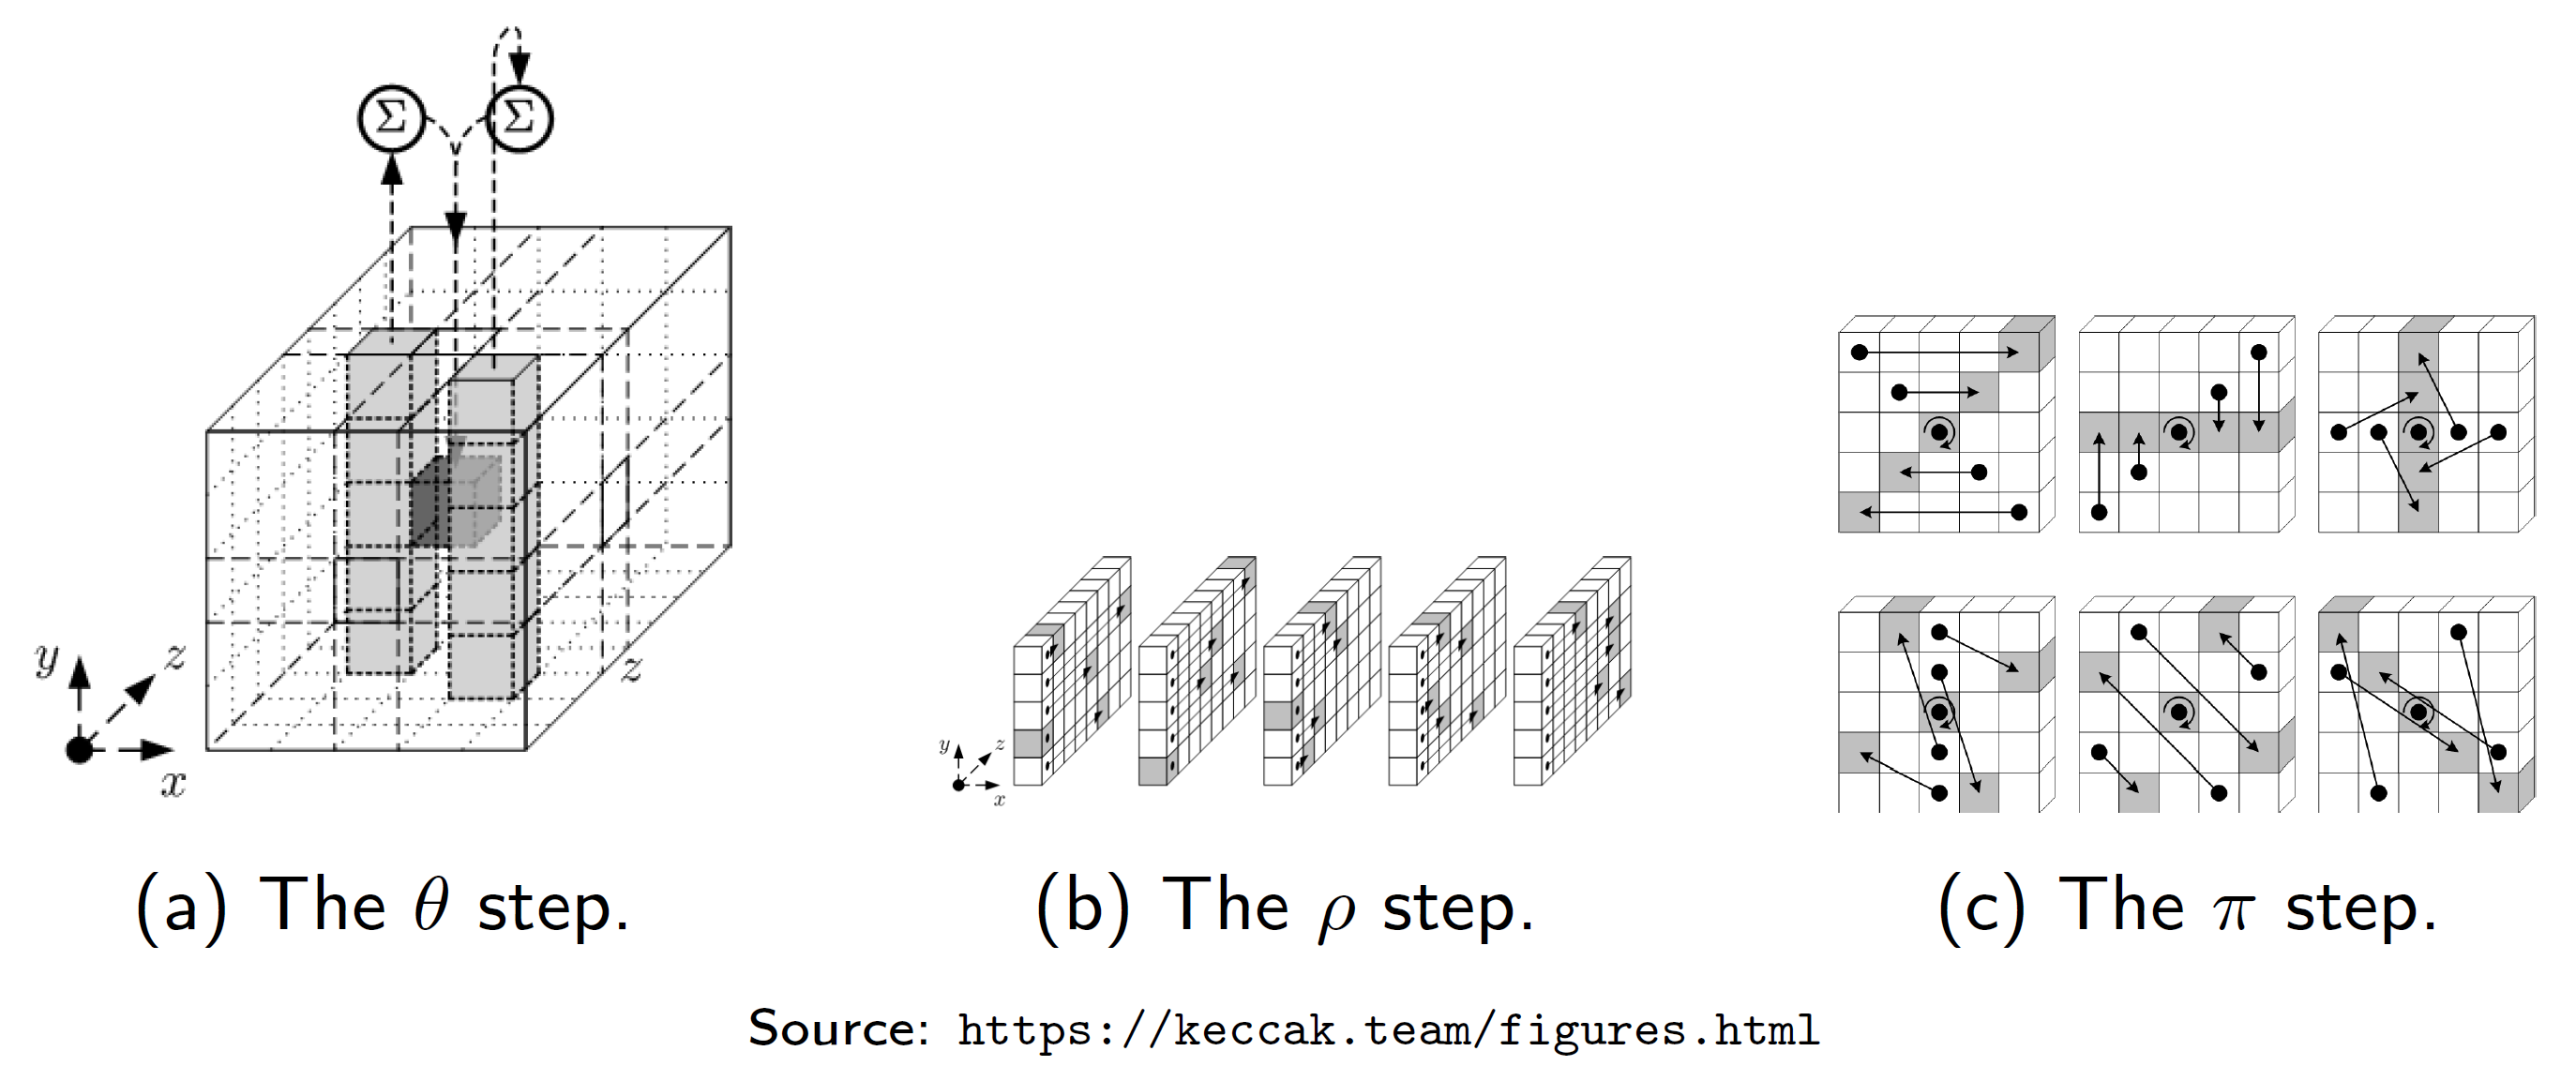
\includegraphics[width=140mm]{Graphics/Hash Functions/hf11.png}
			\end{center}
			\begin{itemize}
				\item Linear mixing layer of the Keccak-f[200] permutation.
				\item Operates similarly for the other variants.
				\item Goal: ensure good diffusion. Similar to the linear layer in block cipher design.
			\end{itemize}
		   	\begin{center}
				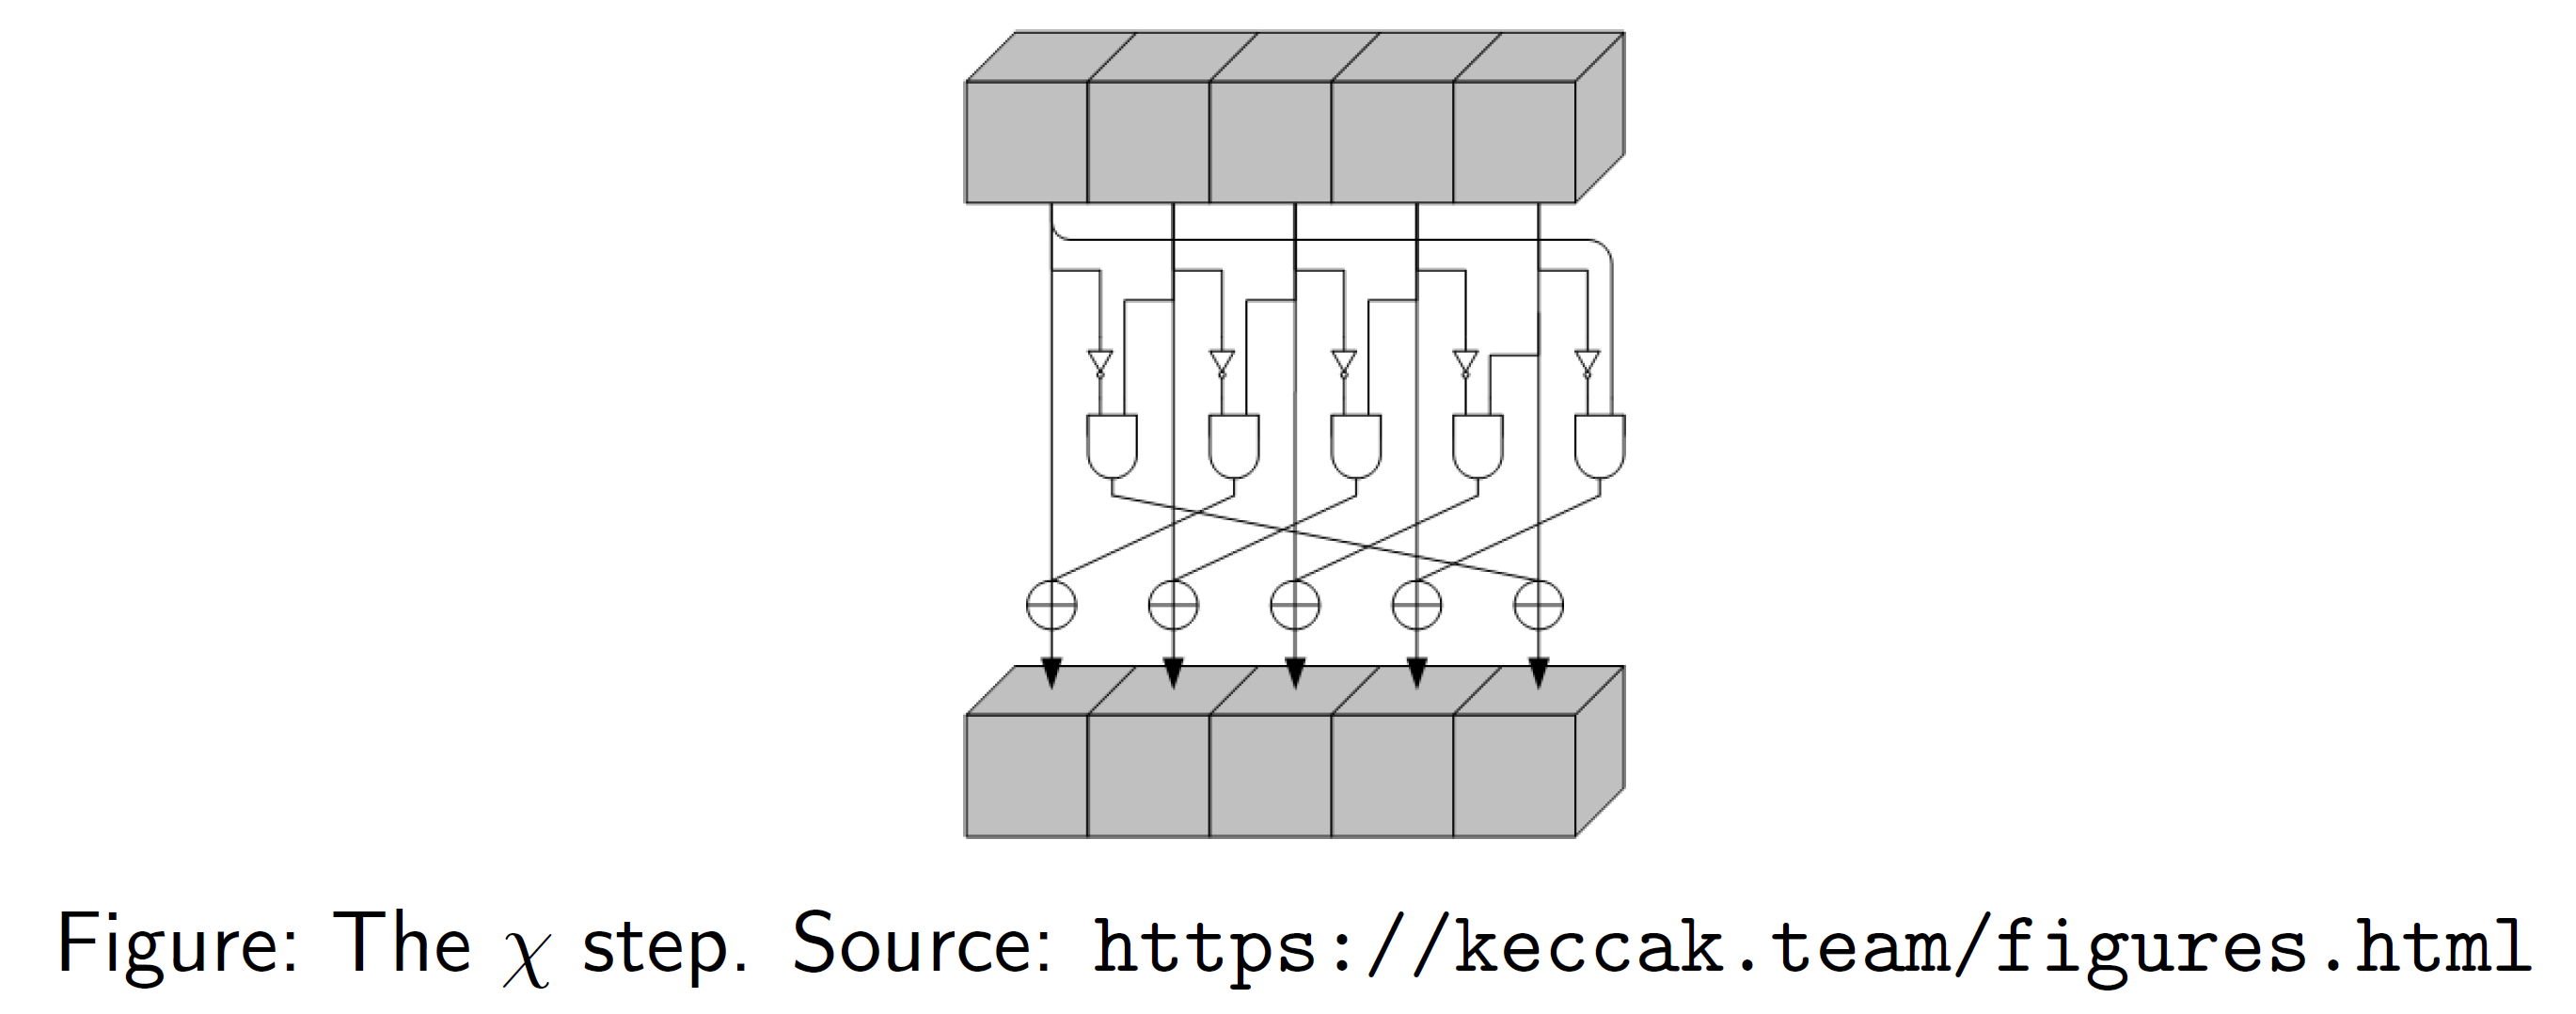
\includegraphics[width=140mm]{Graphics/Hash Functions/hf12.png}
			\end{center}
			\begin{itemize}
				\item Non-linear layer of the Keccak permutation. Operates at the lanes level, but operations are actually bitwise.
				\item Followed by the $\iota$ step: the addition of a round constant to the first lane.
				\item Without $\iota$, the permutation would commute with bitwise rotation of the lanes, and all the rounds would be equal.
			\end{itemize}
		
		\subsubsection{The avalanche effect of the Keccak-f[1600] Permutation:}
			\begin{itemize}
				\item Diffusion property of the linear layer: a 1-bit difference is propagated to 11 different bits then to the input of 11 $\chi$ functions (at the bit level).
				\item Property of the non-linear step: a 1-bit difference in the input of $\chi$ gives at least a 1 bit difference in its output.
				\item Experimental numbers: given a 1-bit difference in input, around half the bits of the state are different at the end of the third round.
			\end{itemize}

\newpage

\section{Cryptanalysis on Hash Functions}
	\subsection{Attacker’s goals against hash functions}
		\begin{itemize}
			\item Recall that a hash function is a map $H: \{0,1\}^* \mapsto \{0,1\}^n$
			\item Possible goals to achieve:
			\begin{itemize}
				\item Collisions: Find distinct bit strings $x$, $y$ such that $H(x)=H(y)$
				\item Pre-image: Given $h \in \{0,1\}^n$, find $x$ such that $H(x)=h$
				\item Second pre-image: Given $x$, find $y \neq x$ such that $H(x) = H(y)$
				\item One-wayness: given a set $S$ of size at most $2^n$ and $h=H(s)$ for $s \in S$.
				Find a $s' \in S$ such that $H(s')=h$
			\end{itemize}
			\item Of all these goals, collisions is usually the easiest to attack
		\end{itemize}
		Hash functions are widely used in cryptography. 
		So much that they are sometimes referred to as the cryptographic swiss-knife. 
		Because of this, they need to satisfy several essential properties. 
		From the point of view of the attacker, this gives more attack targets. 
		The most well-known target is the search for collisions where the attackers looks for two different strings that hash to the same value. 
		Then we find the search for pre-images where he needs to find a message that hashes to a given target. 
		There are two frequent variations on this. 
		Second pre-images, where given a message the attacker needs to find a distinct message with the same hash value. 
		And one-wayness, where given the hash of a message from a relatively small set, he has to find a message from the same set hashing to the prescribed value. 
		In that case, the original message is the desired target but any other message that collides with it is also accepted.\\
		Among these goals, finding collisions is usually the easiest, and it will be our main topic during the lecture.
	
	\subsection{Random Oracle Model}
		\begin{center}
			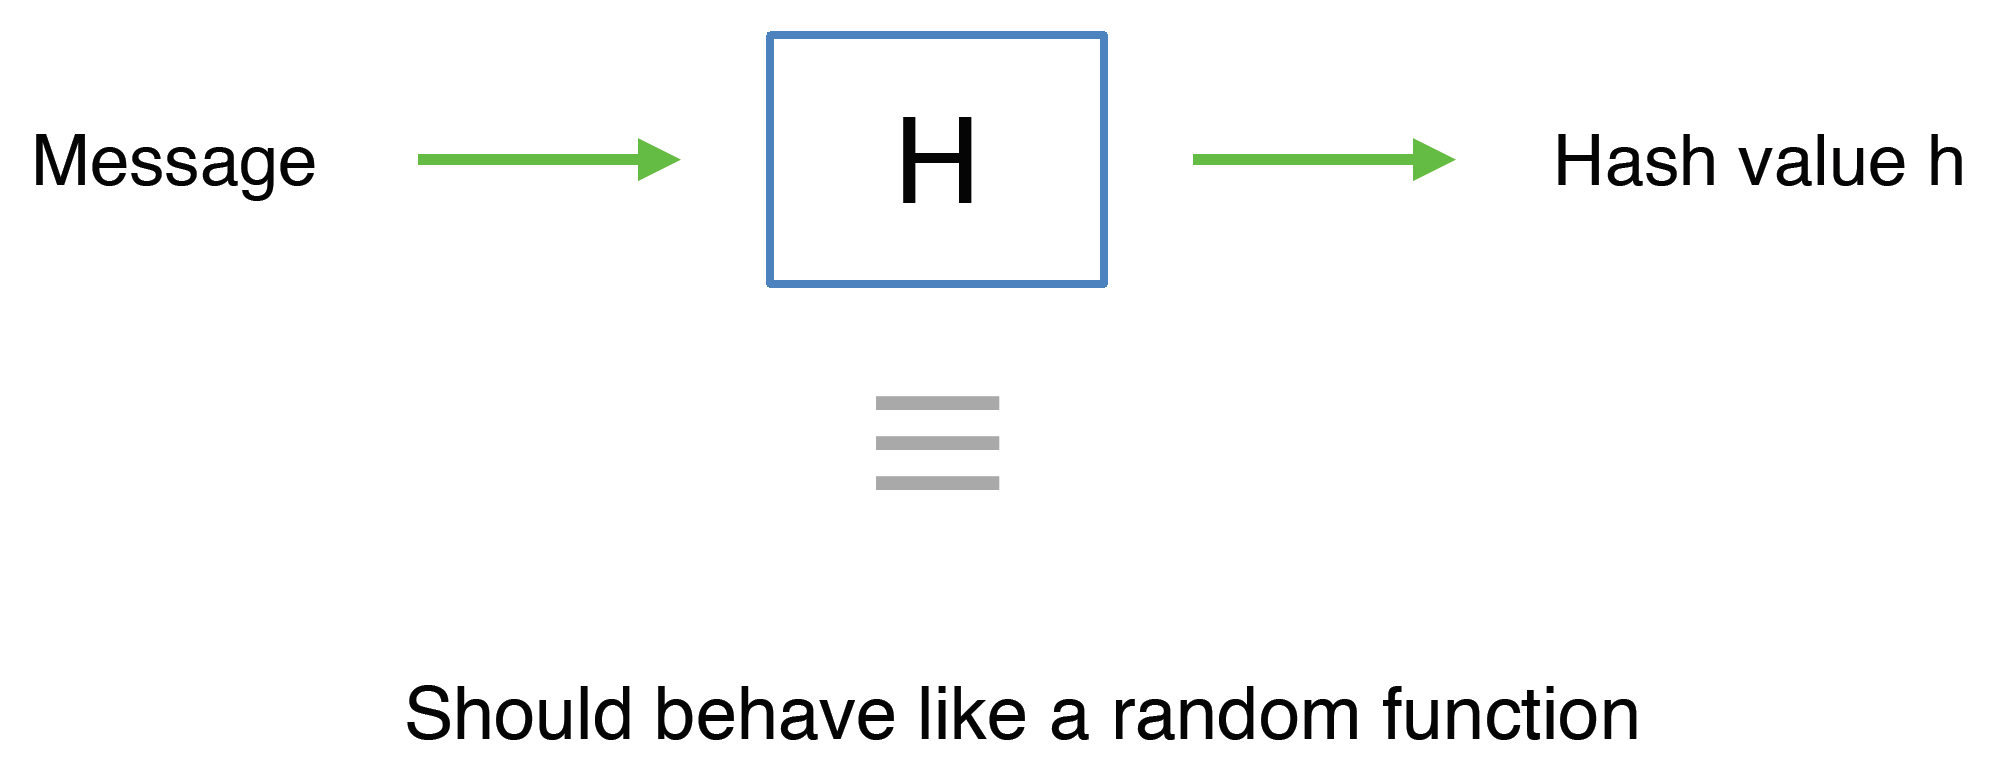
\includegraphics[width=120mm]{Graphics/Hash Functions/hf13.png}
		\end{center}
		A frequently encountered idealisation of hash functions is the random oracle model where the output value is chosen uniformly at random for every new message. 
		(Of course, since hash functions are deterministic, the answer to an already asked question should remain identical). 
		In other words, the hash function should behave like a random function. 
		This is impossible to achieve, since a random function almost never has a short description as a computer program, while a hash function does by design.\\
		As a consequence of this it is possible to construct cryptographic protocols that are secure when using a random oracle but become insecure as soon as it is replaced by any concrete hash function.
		Admittedly, these examples are contrived and the random oracle model remains a good way to create sound designs.
	
	\subsection{Generic Collisions}
		\begin{itemize}
			\item The key ingredient is the \textit{birthday paradox}
			\item If we have a set of size $N$ and random elements:
			\begin{itemize}
				\item Collision guaranteed after picking $N+1$ (pigeonhole principle)
				\item Collision with constant probability after $\mathcal{O}(\sqrt{N})$
				\item Collision with overwhelming probability after $\mathcal{O}(\log N \cdot \sqrt{N})$
			\end{itemize}
		\end{itemize}
		Even with idealised hash functions, collisions are possible. 
		Indeed, the set of possible messages is infinite while the set of hashed values is finite, as a consequence, collisions must exist. 
		In fact, if the size of the set of hashed values is $N$, a collision is guaranteed as soon as we have hashed $N+1$ messages. 
		This is the pigeonhole principle and it also holds for randomly chosen values.\\
		However, and may be surprisingly, it is possible to do much better. 
		If we only want a collision to occur with constant probability or even with overwhelming probability, we only need to consider 
		a number of messages of the order of square-root of $N$ or slightly larger.\\
		This fact is usually known as the birthday paradox because it applies when looking for people with common birthday in a relatively small group.
	
	\subsection{Explanation of birthday paradox}
		\begin{itemize}
			\item Picking $s$ elements in $N$
			\begin{itemize}
				\item Number of ordered choices (with collision): $N^s$
				\item Number of ordered choices (without collisions): $\frac{N!}{(N-s)!}$
			\end{itemize}
			\item Example for $N=365$:
		\end{itemize}
		\begin{center}
			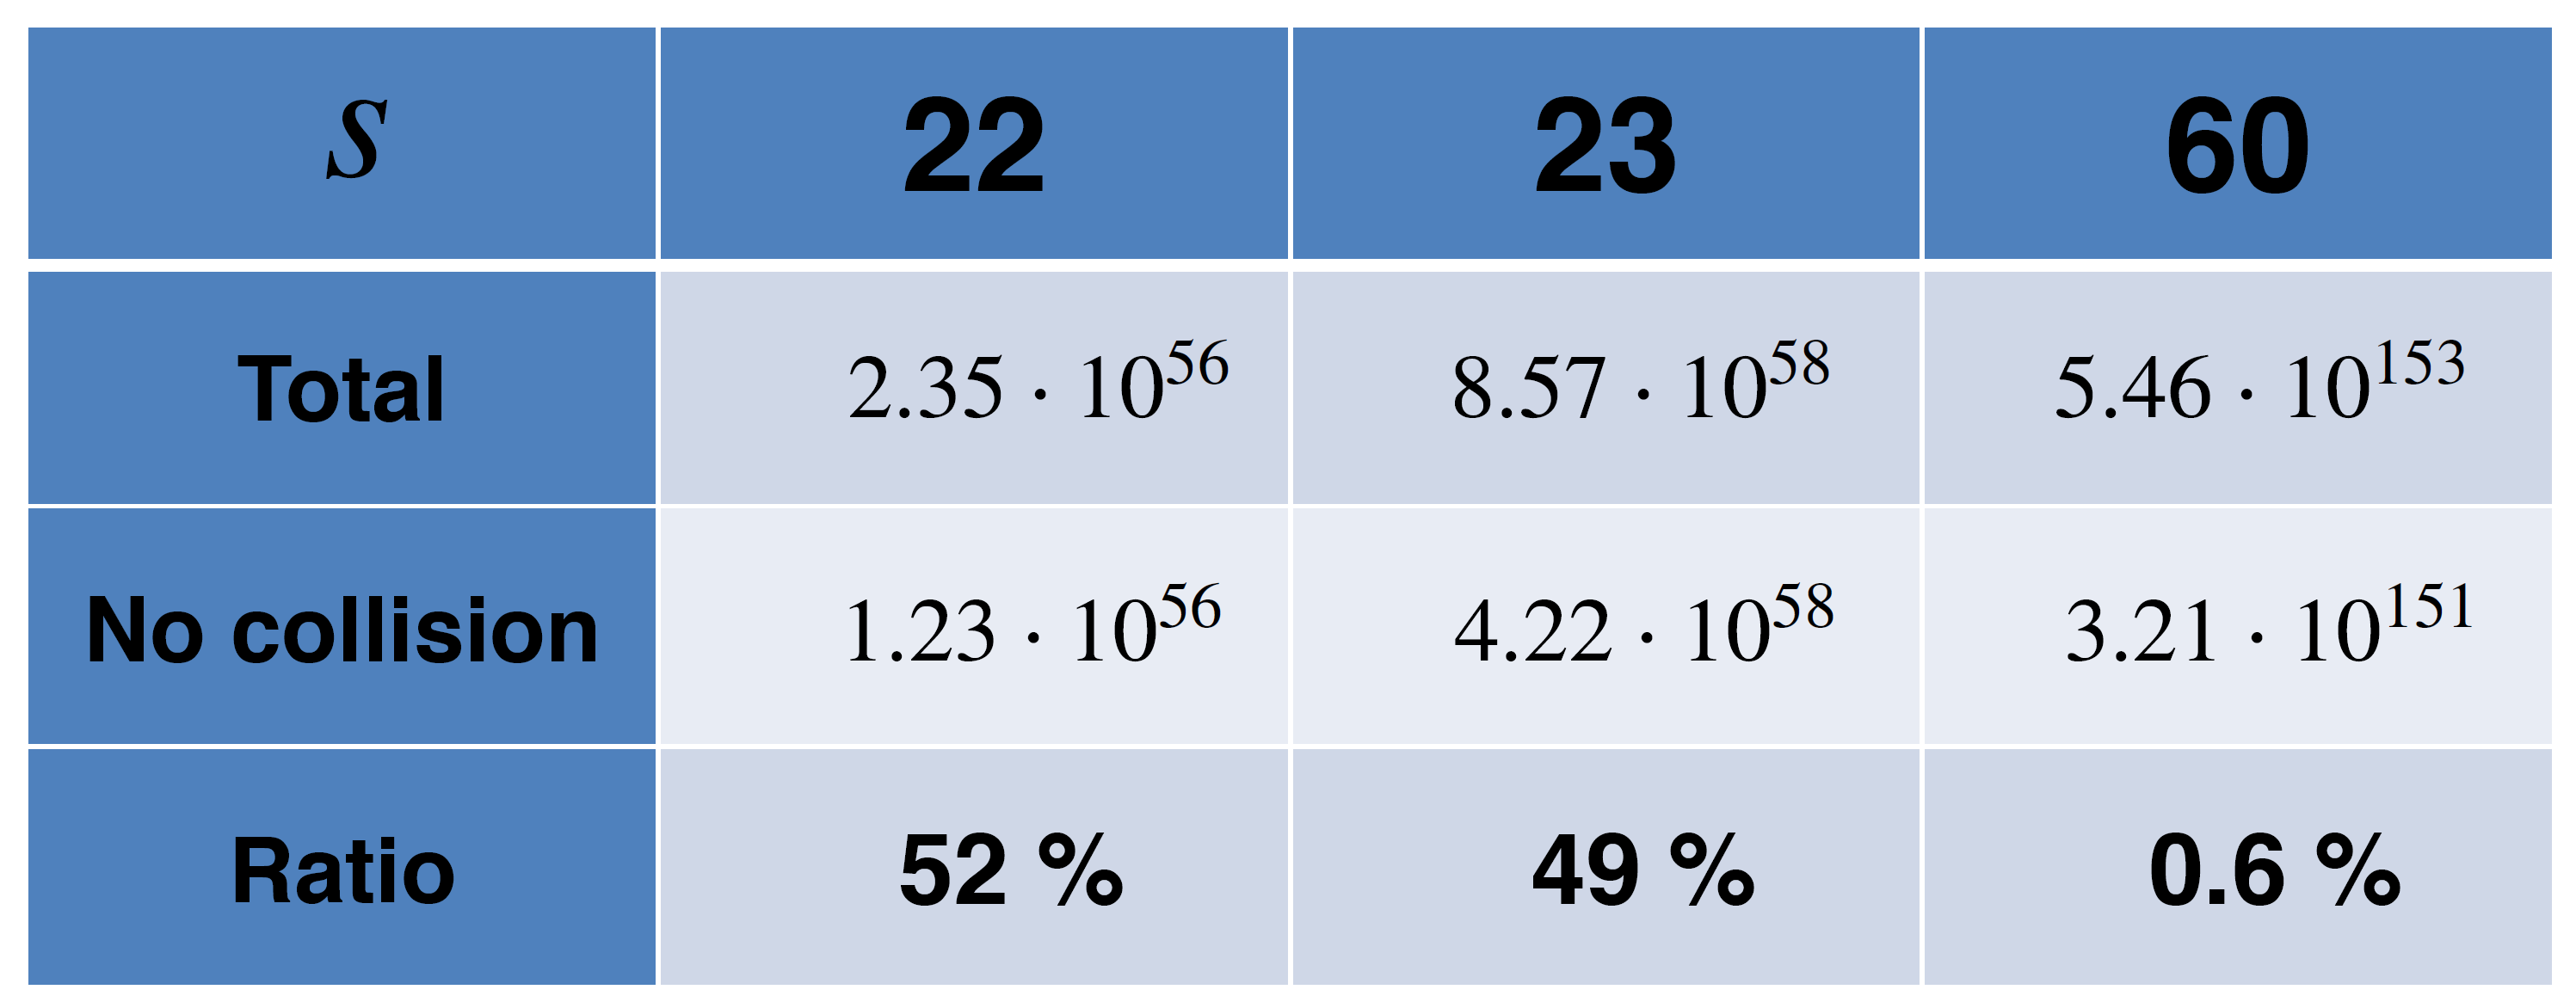
\includegraphics[width=120mm]{Graphics/Hash Functions/hf14.png}
		\end{center}
		The reason for this is combinatorial in nature. 
		Assume that we are picking $s$ elements in a group of $N$. 
		The number of possible ways of choosing is $N$ to the $s$, if duplicates are permitted. 
		If they are not, they are fewer options, namely $N$ factorial over $(N-s)$ factorial.
		Let’s do the concrete computations for $N=365$, i.e., for the case of birthdays (omitting leap years). 
		For $s=22$, we see that about $52\%$ of the cases are without collisions and for $s=23$, only $49\%$ are without collisions. 
		As a consequence, the probability of getting a collision is higher than one half. 
		Furthermore, for $s=60$, the probability is higher than $99\%$ (of getting a collision).
		\begin{itemize}
			\item We can simplify the probability as:
				$$p(s) = \prod\limits_{i=0}^{s-1} \frac{N-i}{N}$$
			\item Remember that
				$$ln(1-x) \leq -x \  \text{(for all} \  x<1 \text{)}$$
			\item Taking logarithm we have:
				$$ln(p(s)) \leq -\sum\limits_{i=0}^{s-1} \frac{i}{N} = -\frac{s(s-1)}{2N}$$
		\end{itemize}
		To show this, we can rewrite the probability of not having a collision as $N$ factorial over $(N-s)$ factorial divided by $N$ to the $s$. 
		Rearranging terms, we get the product of value $N-i$ over $N$ for $i$ ranging from $0$ to $s-1$. 
		Taking $log$, we turn this into a sum. 
		Remembering that the $log$ of $(1-x)$ is always smaller than $-x$, we can upper bound the $log$ of the probability of not having a collision by $-s(s-1)$ over $2N$. 
		When s becomes bigger than square root of $N$, this bound becomes a negative constant and the probability of not having a collision is bounded away from $1$. 
		Furthermore, if $s$ is of the form square root of $N$ times $log(N)$, the bound tends to minus infinity and the probability of not having 
		a collision becomes as close to $0$ as we desire when $N$ grows. 
		In other words, the probability of having a collision is overwhelming.
	
	\subsection{An example scenario for exploiting collisions: digital signature}
		\begin{itemize}
			\item In the standard Hash-and-sign paradigm
		\end{itemize}
		\begin{center}
			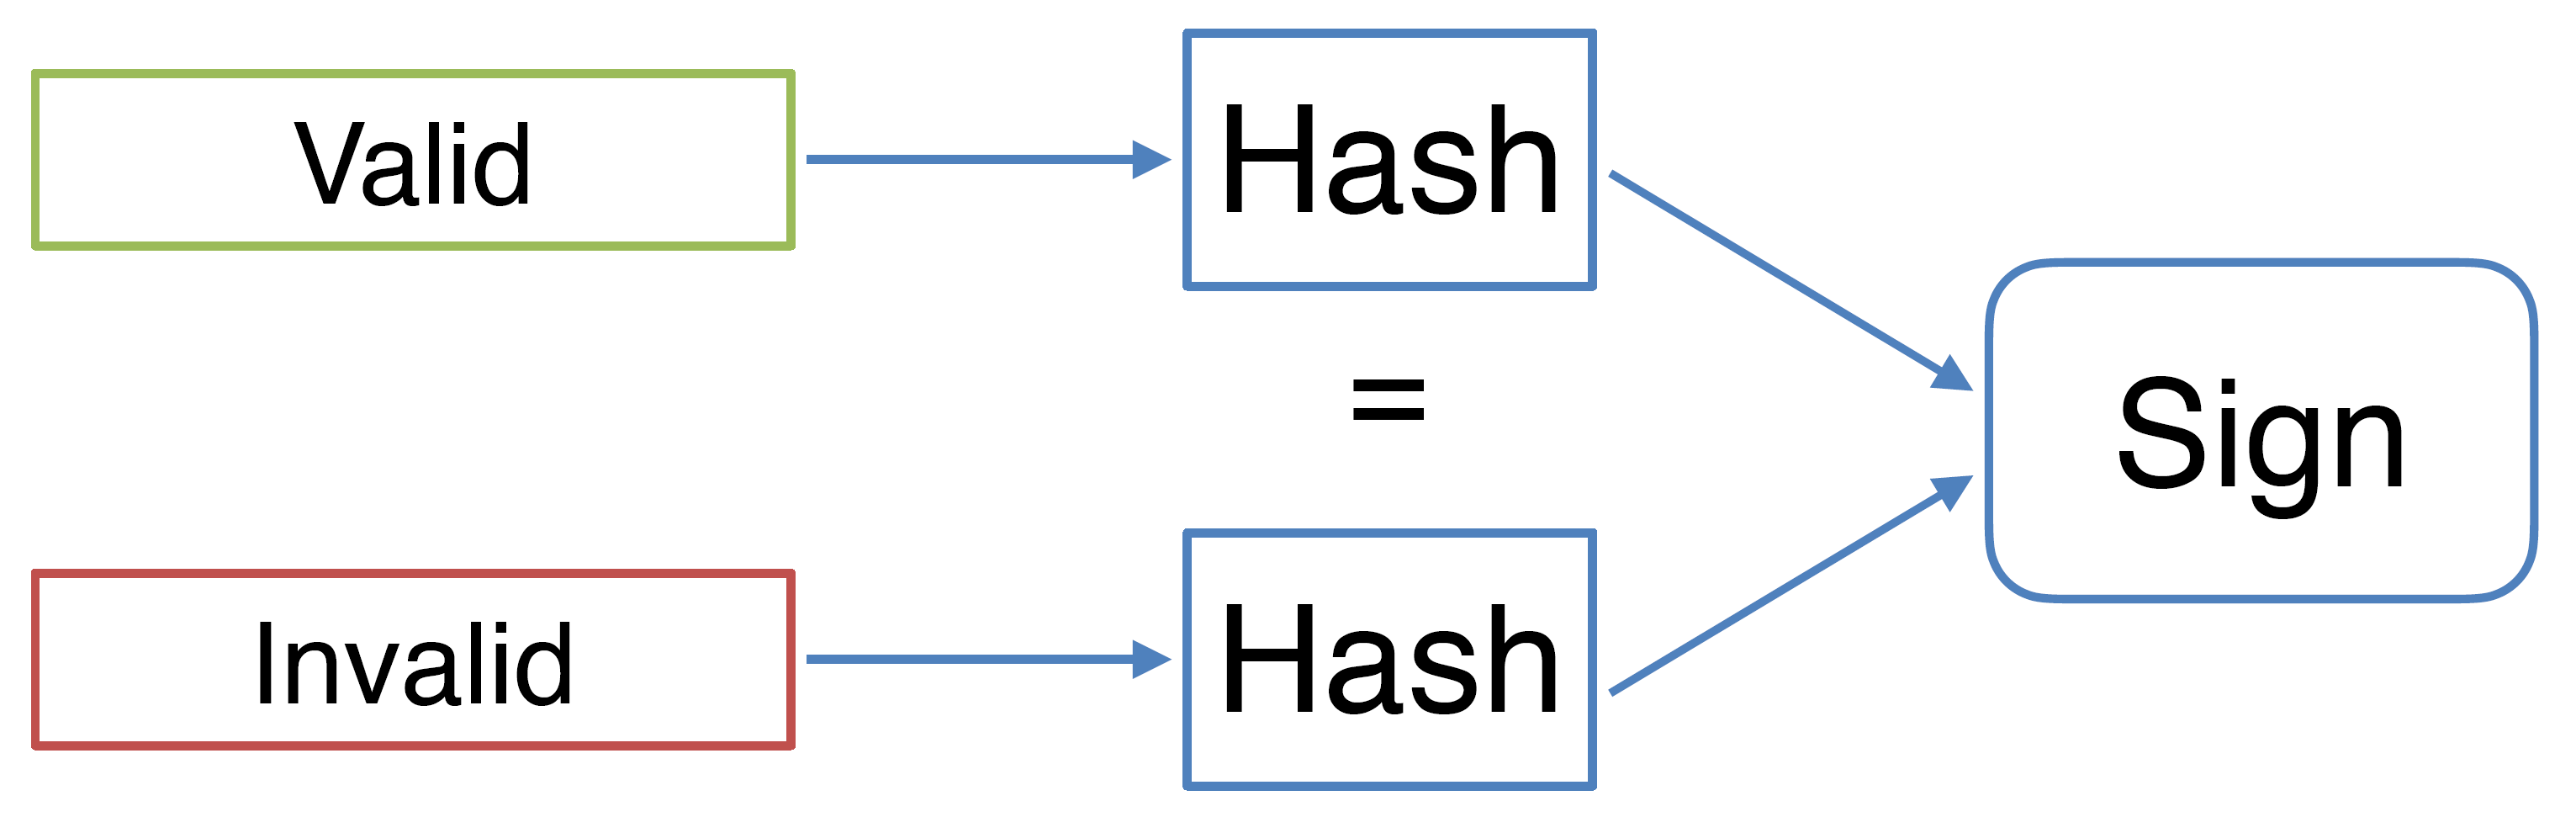
\includegraphics[width=120mm]{Graphics/Hash Functions/hf15.png}\\
			Hash collision can thus lead to signed unwanted messages
		\end{center}
		Collisions can, in particular, be used to forge digital signatures. 
		Indeed, if an attacker can prepare two messages with the same hash value, one of which can be accepted as valid by the signer while the other would be rejected, 
		then (in the classical hash-and sign paradigm) he can use the signature obtained for the valid message and pretend that it is a signature of the other one. 
		This is clearly a forgery.
	
	\subsection{More details}
		\begin{center}
			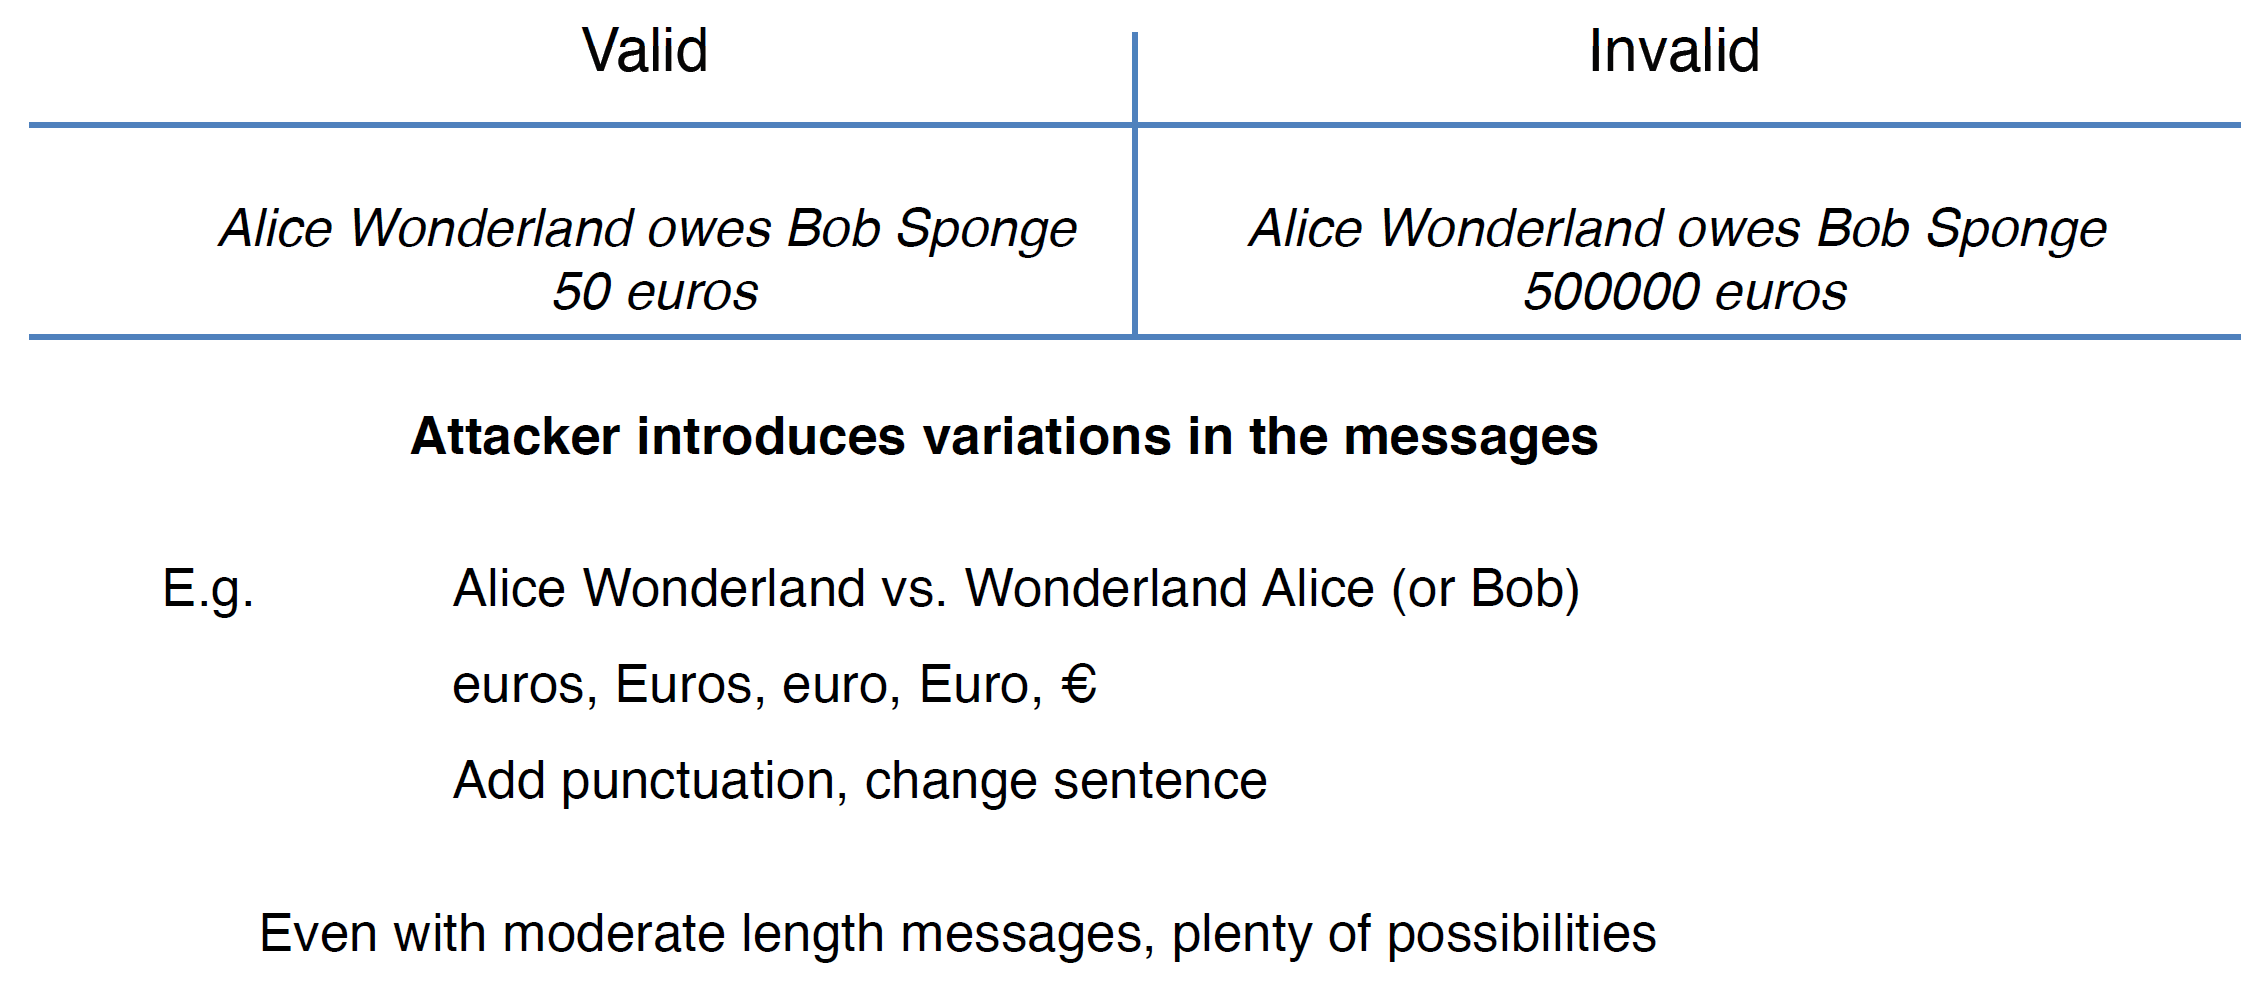
\includegraphics[width=120mm]{Graphics/Hash Functions/hf16.png}
		\end{center}
		In practice, preparing messages for the attack relies on the fact that given a message in a natural language, 
		it is possible to create plenty of variations of the message without altering its meaning. 
		In our example, Alice is ready to sign a letter saying that she owes Bob 50 euros. 
		However, Bob want to change that to half a million. 
		We show on the slide a few ways of changing the sentence without changing its meaning. 
		The good thing for the attacker is that changes are mostly independent which means that the number of variation are multiplied. 
		In particular, identifying 40 places in the message where 4 variations are possible is enough to get $2^{80}$ variations. 
		By the birthday paradox, this would be enough to be able to find collisions for 160 bit hash functions. 
		Of course, the computational cost for Bob to perform this generic attack would be high.\\
		This size of 160 bits was the standard for a long time and was used in the SHA-1 hash function. 
		Nowadays, 256 bits or even 512bits are preferred.
	
	\subsection{Memory-less collision finding}
		\begin{itemize}
			\item Also a major algorithmic tool in cryptanalysis
			\item Consider a random function $f: S \mapsto S$
			\item We want a collision $f(s) = f(s')$
			\item Pick random and build sequence $s_{i+1} = f(s_i)$
			\item Since is finite, the sequence is ultimately periodic
		\end{itemize}
		\begin{center}
			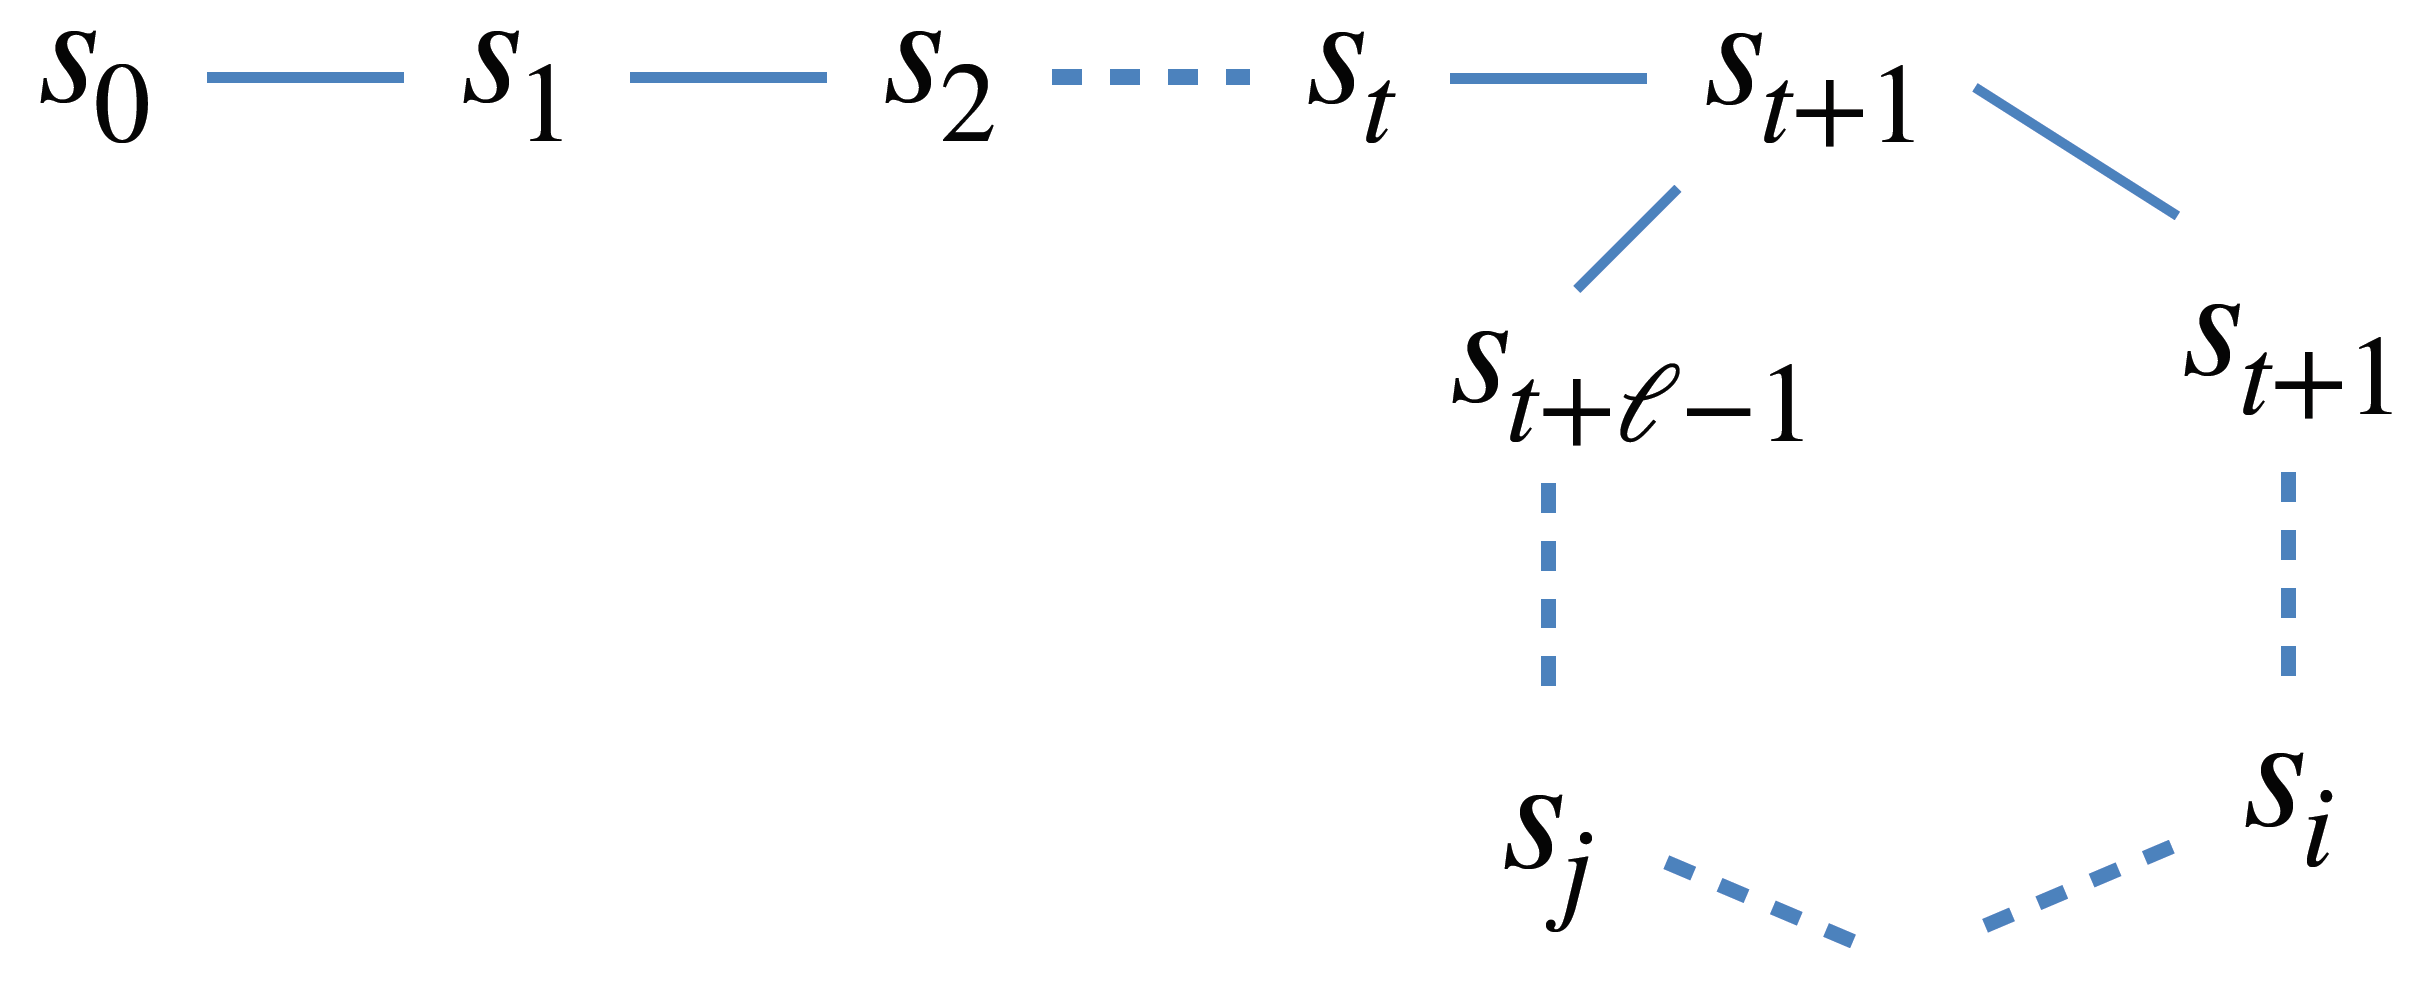
\includegraphics[width=120mm]{Graphics/Hash Functions/hf17.png}
		\end{center}
		We saw in the block cipher cryptanalysis lecture that collisions can be found quickly using fast sorting techniques. 
		However, this approach requires a lot of memory and this memory cost is usually the limiting factor for the attacker. 
		We now consider the problem of finding collisions without using large amounts of memory.\\
		We assume that $f$ is a random function from a set to itself and we search for a collision $f(s)=f(s’)$.\\
		The trick is to start from a random point $s_0$ and consider the sequence defined by the recursive formula $s_(i+1)=f(s_i)$. 
		Of course, since the sequence is infinite, the values it takes must cycle back at some point. 
		Note that, there is no reason, in general, to cycle back to $s_0$ and most of the time, the sequence looks that the picture on the slide. 
		There is a tail, followed by a cycle and the sequence is ultimately periodic.\\
		It is clear that the entry point in the cycle has two distinct pre-images, one in the cycle and one in the tail. 
		Thus, there is a collision at this location.\\
		We now need an algorithmic technique to efficiently find this entry point and compute the collision.
		\begin{itemize}
			\item We want to find the entry points to the cycle
			\item Without storing all intermediate computations
			\item Many methods, we consider Floyd’s cycle finding technique\\
			\item Idea: Compute in parallel $s_n$ and $s_{2n}$
			\begin{itemize}
				\item At some point, we will get a collision $s_n = s_{2n}$, with $l|n$
				\item We thus obtain a multiple of $l$\\
			\end{itemize}
			\item Then, we use it to reconstruct the entry points.
		\end{itemize}
		There are several algorithms to do that, but they all share the same principle. 
		First, identify the length of the cycle (or a multiple of it) and then recover the entry points. 
		We only consider Floyd’s algorithm that find the cycle’s length by computing the sequences $s_n$ and $s_{2n}$ in parallel.\\
		Note that this can be done using only a small amount of memory. 
		Indeed, $s_n$ is computed just by applying $f$ to the previous value and $s_{2n}$ by applying $f$ twice to $s_{2*(n-1)}$. 
		We will refer to them as the slow and fast sequences.\\
		Keeping in mind the picture from the previous slide, we see that the fast sequence rushes ahead and enter the cycle much earlier than the slow one. 
		Of course, once in the cycle, the sequence stays there and waits for the slow sequence to also enter the cycle. 
		Once they are both in it, we can view the fast sequence as being behind the slow one and we see that at each moment in time it gets closer to it by one step. 
		Thus, at some point, the fast sequence catches the slow one and we have $s_{2n}=s_n$. 
		When this happen, $n$ is necessarily a multiple of the cycle length.\\
		In the next slide, we show how to use the length to get the collision itself.
		\begin{itemize}
			\item Given a multiple $L$ of $l$, construct the entry point
			\begin{itemize}
				\item Step 1: Compute $s_L$
				\item Step 2: Compute in parallel $s_i$ and $s_{L+i}$ until $s_i = s_{L+i}$
				\item Then, $f(s_{i-1}) = f(s_{L+i-1})$ is the desired entry point collision
			\end{itemize}
		\end{itemize}
		Once we have a multiple of the length of the cycle (call it $L$), we first compute $S_L$ then maintain in parallel the two sequences $s_i$ and $s_{L+i}$. 
		At some point, precisely when $i$ is the length of the tail, the two sequences collide and we discover a collision for $f$.\\
		Analysing these cycle finding techniques isn’t a trivial matter, however, the conclusion is they also have a running time of the order of the square of the size of the set $S$. 
		As a consequence, whenever possible, this method should be preferred to collision finding with memory.
	
	\subsection{Generic pre-images, second pre-images and one wayness}
		\begin{itemize}
			\item Basically, use exhaustive search.
			\item For Pre-images the expected time is the size of the output set
			\item For One-wayness it is the minimum of the size of output and reference sets
		\end{itemize}
		For pre-images or one-wayness, generic attack basically rely on exhaustive search. 
		It simply consists of trying distinct messages until the desired target is reached. 
		For pre-images, the expected time is the size of the output set. 
		For one-wayness, assuming the initial message whose hash value is given belongs to a smaller set, it suffices to try all the messages in that smaller set to succeed.
	
	\subsection{Parallel Hash extension}
		\begin{center}
			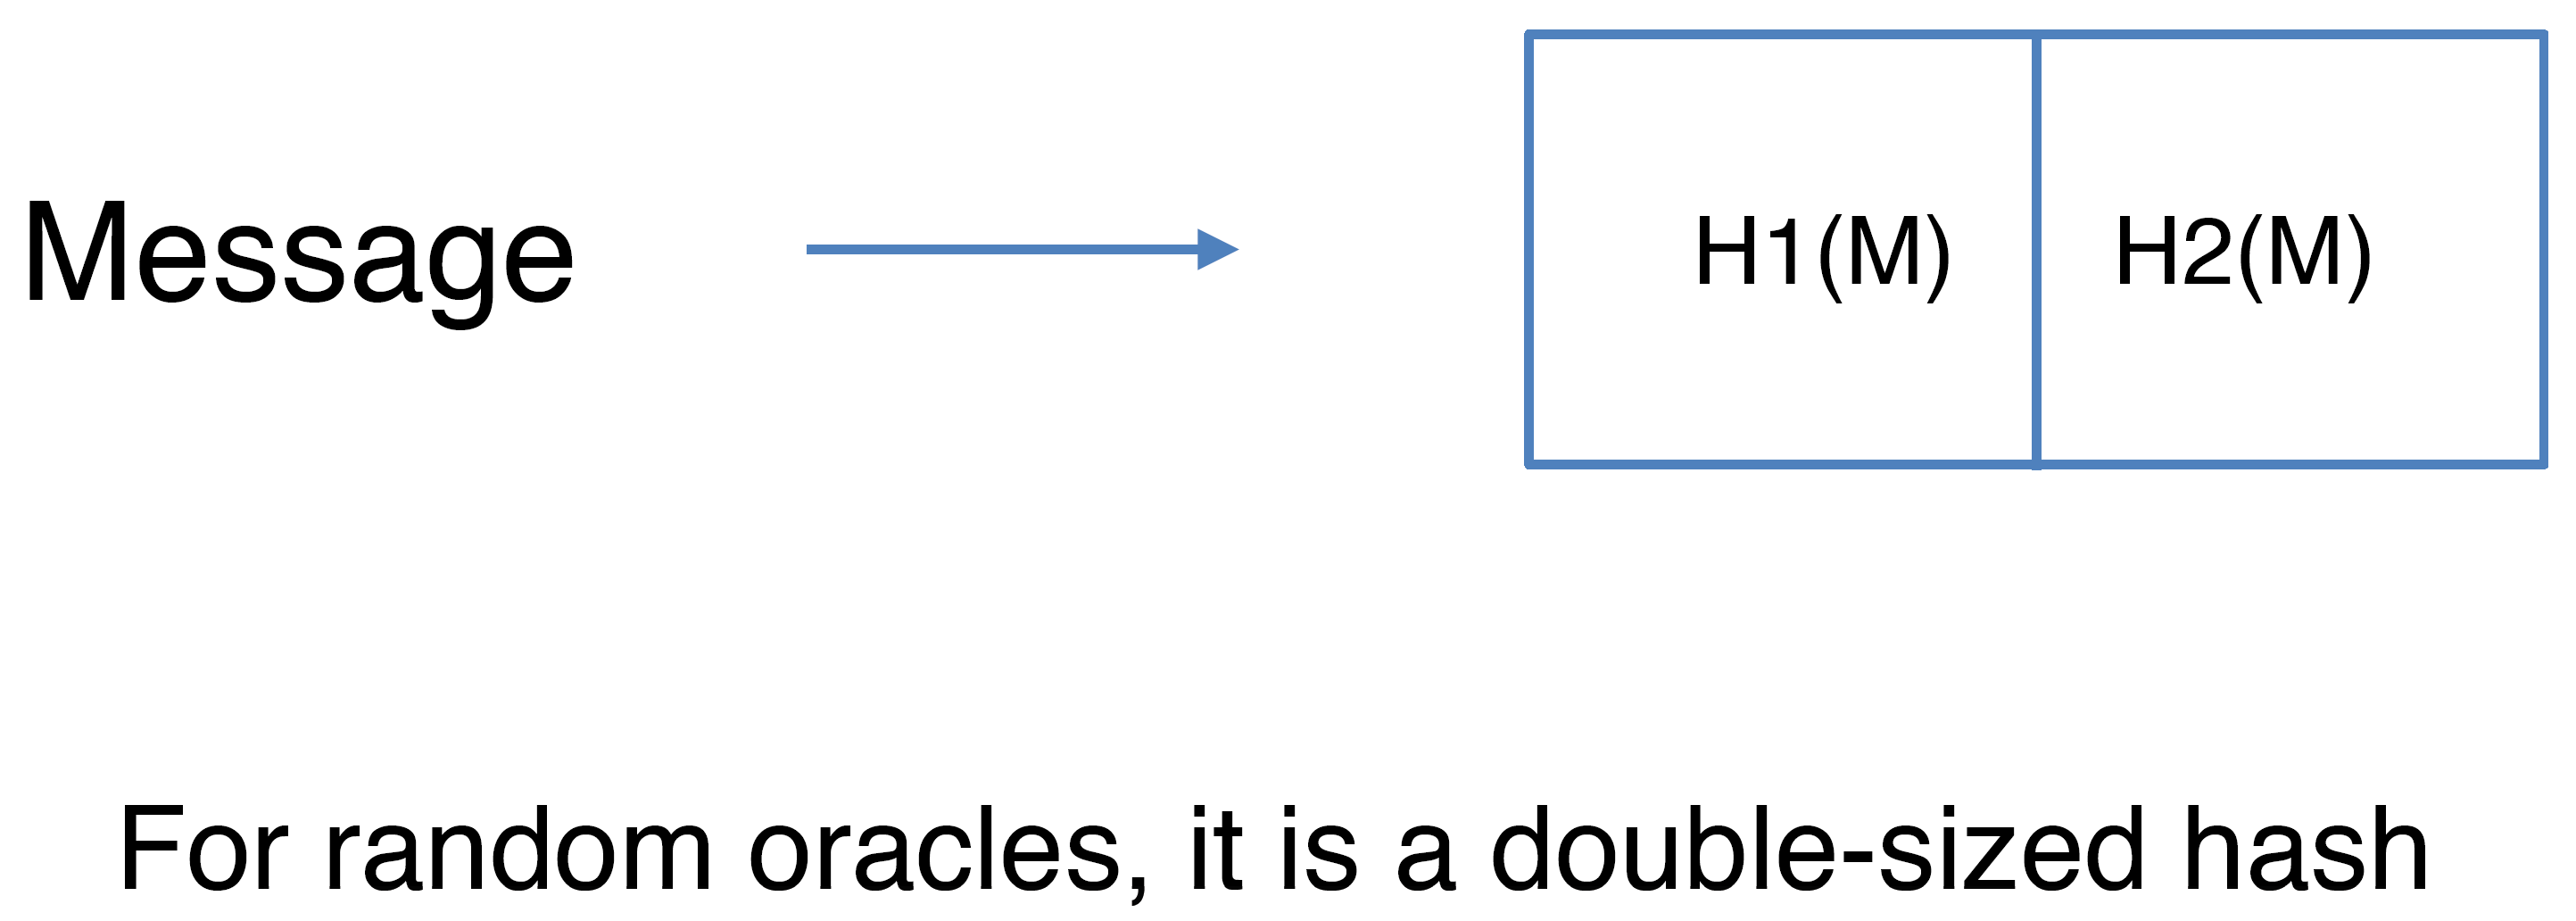
\includegraphics[width=120mm]{Graphics/Hash Functions/hf18.png}
		\end{center}
		We now move into the realm of non generic attacks and show a construction that despite being generically secure can fail utterly in practice. 
		This construction is the parallel hash extension method. 
		Assume that we have two hash functions $H_1$ and $H_2$ on $n$ bits each and look at the function that given a message $M$ put together $H_1(M)$ and $H_2(M)$. 
		It is easily shown that if $H_1$ and $H_2$ are random oracles on $n$ bit each then this parallel composition (also called concatenation) is a random oracle on $2n$ bits. 
		As a consequence, this technique was long consider to be a nice way to build large hash functions from smaller ones. 
		Of course, it is clear that there are bad choices such as $H_1 = H_2$ and people guessed that having $H_1$ and $H_2$ too similar wouldn’t be a good idea.\\
		We are now going to show why this fails as soon as $H_1$ is a Merkle-Damgard hash function.
		
	\subsection{Merkle-Damgard Hash construction}
		\begin{center}
			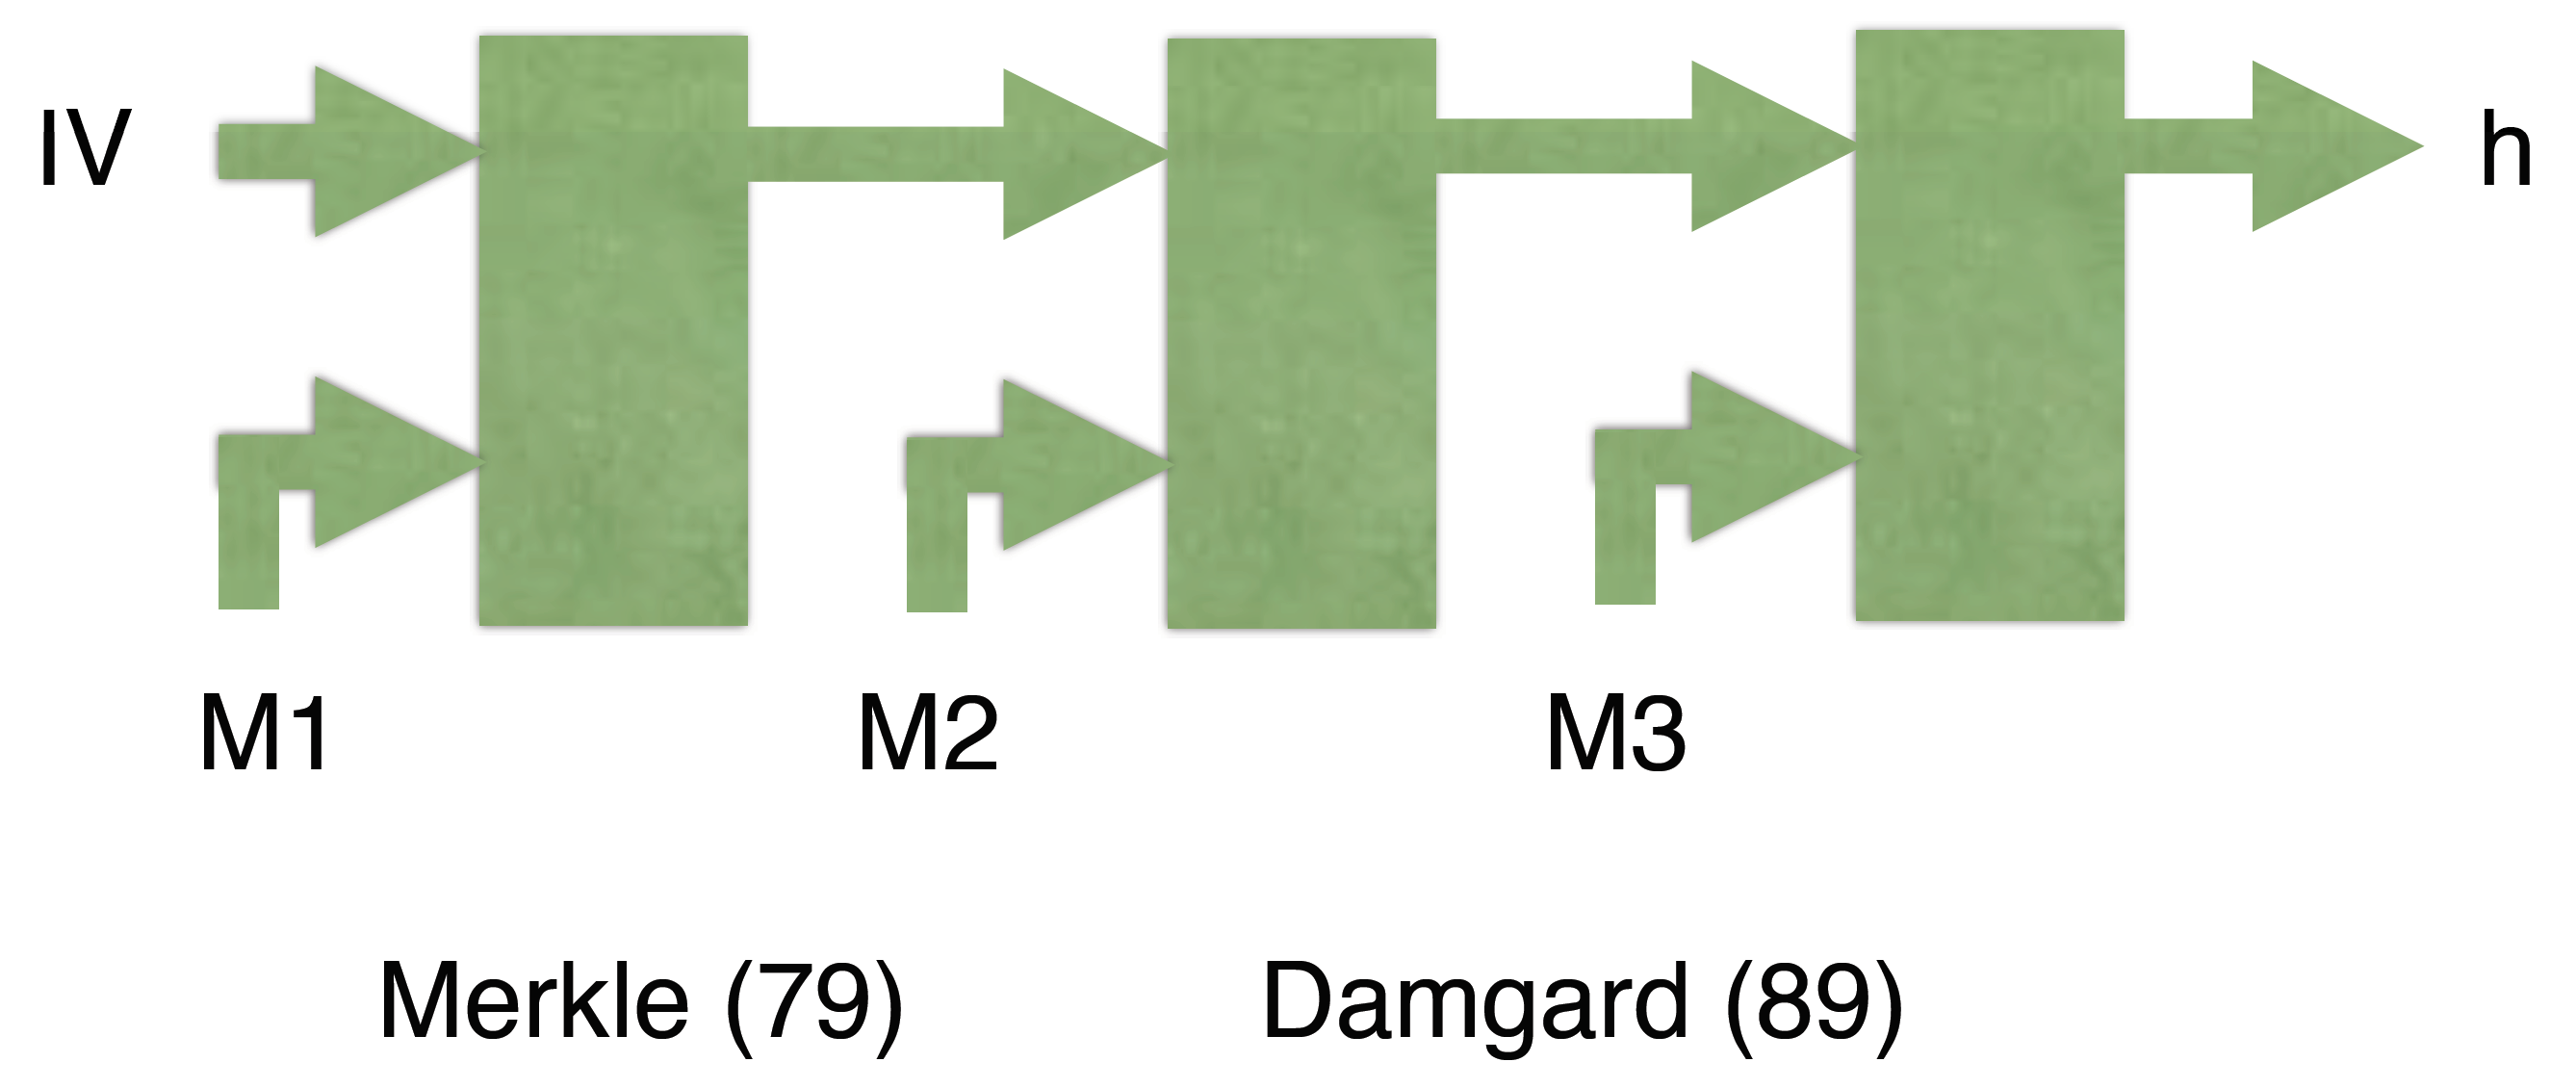
\includegraphics[width=120mm]{Graphics/Hash Functions/hf19.png}
		\end{center}
		We briefly recall that a Merkle-Damgard hash is based on a compression function and computes the hash block by block starting 
		from a fixed initial value and compressing at each round the current value and a message block into a new value. 
		The final value is the hash result.\\
		Note that the message is pre-formatted by using padding techniques to make its length a multiple of the block size.\\
		For simplicity, we assume in the sequel that the blocks are of size at least comparable to the inner values.
	
		\subsubsection{Multicollisions on Merkle-Damgard construction}
			\begin{center}
				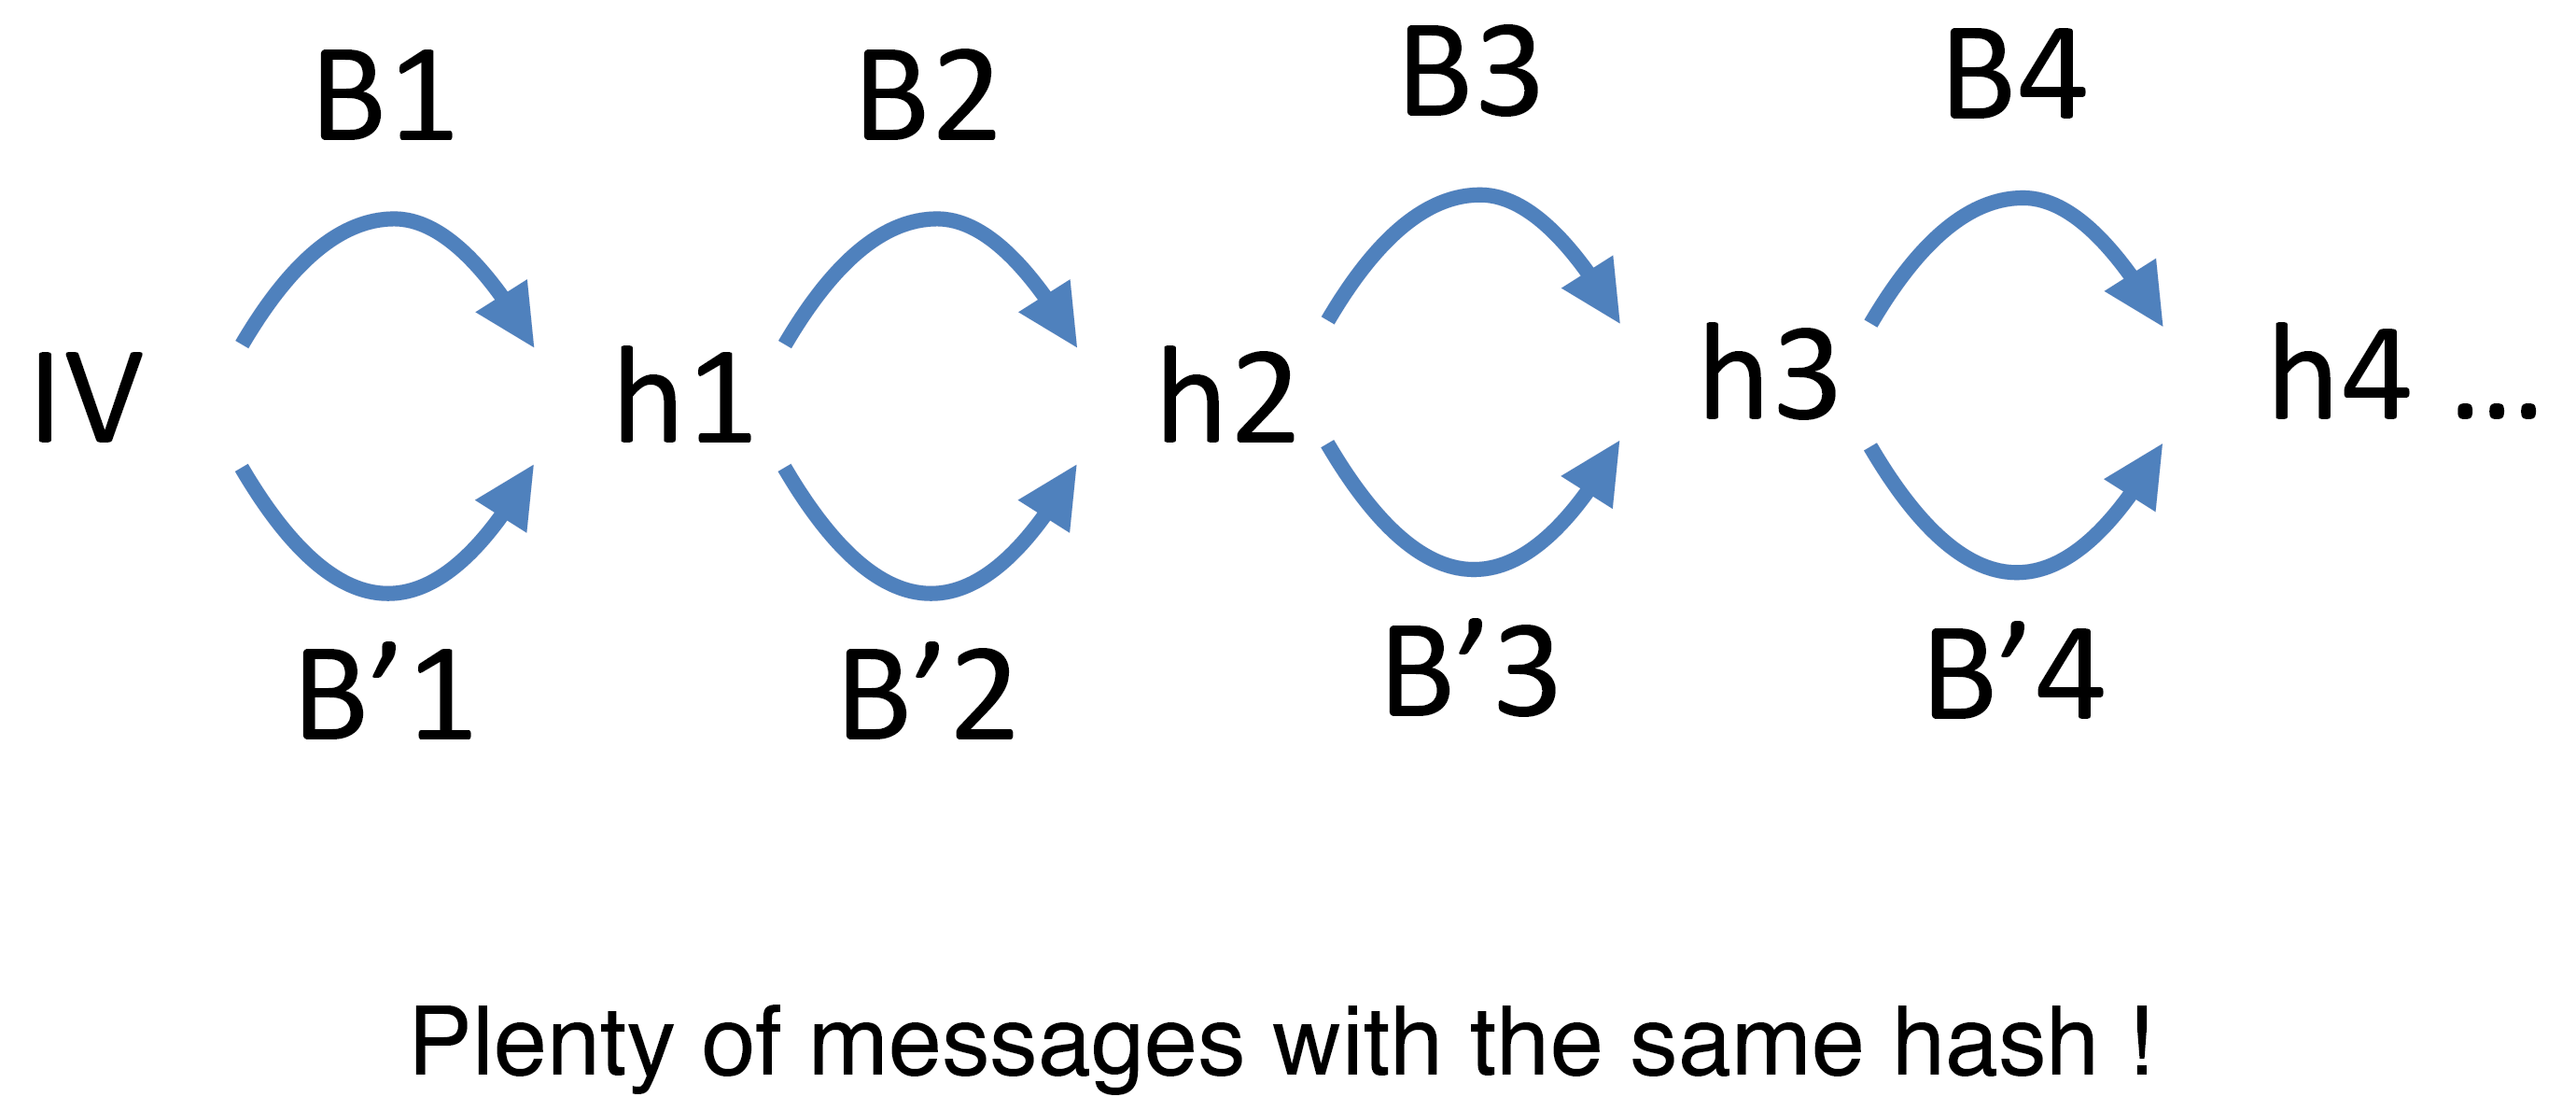
\includegraphics[width=120mm]{Graphics/Hash Functions/hf20.png}
			\end{center}
			Since the blocks are large enough and thanks to the birthday paradox, there should be two blocks $B_1$ and $B'_1$ such that the first compression step collides, giving an internal value $h_1$.
			Similarly we can find two block $B_2$ and $B'_2$ such that the compression of $h_1$ and the block collides giving $h_2$.\\
			If we continue like this, we can create plenty of distinct messages with the same hash. 
			On our example with four blocks, we have 16 distinct messages built by taking an arbitrary mix of the four $B/B’$ blocks. 
			Working with $t$ blocks instead of 4, we would obtain a set of $2^t$ colliding messages for $t$ times the cost of one collision.\\
			Such structures are called multi collisions on the hash function and they are extremely hard to construct on random oracles.
		
		\subsubsection{Parallel Hash extension with a Merkle-Damgard hash}
			\begin{center}
				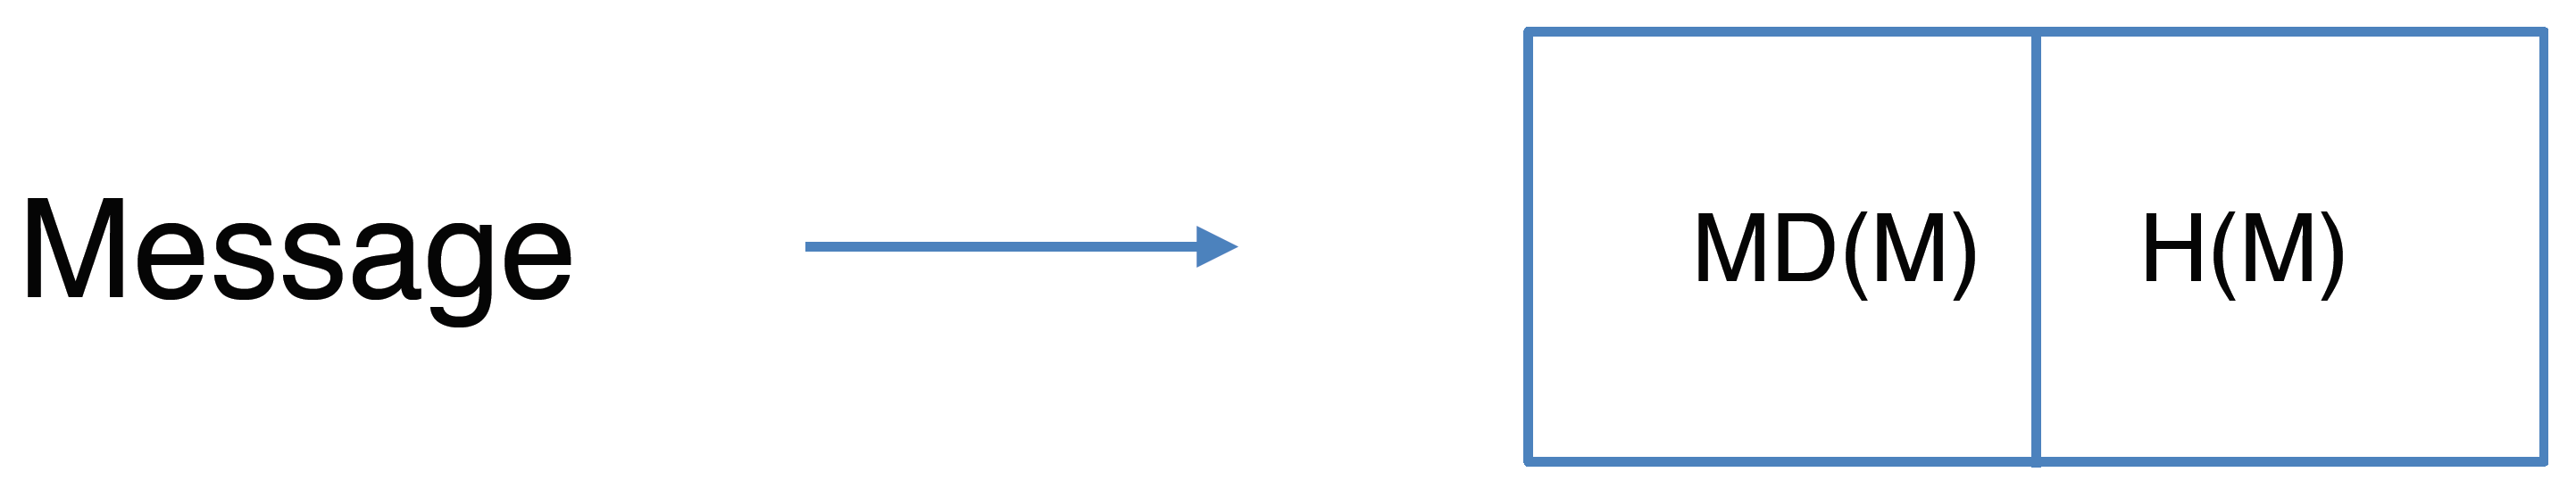
\includegraphics[width=120mm]{Graphics/Hash Functions/hf21.png}
			\end{center}
			For the MD part, construct a multicollision with $2^{\frac{n}{2}}$ messages.
			Then, by birthday paradox, find a collision on $H$.
			Global cost much closer to $2^{\frac{n}{2}}$ than to $2^{n}$.\\
			
			We now come back to the parallel extension where $H_1$ is a Merkle-Damgard hash function. 
			We first construct a multi collision of size $2^{\frac{n}{2}}$ on this hash. 
			Among these $2^{\frac{n}{2}}$ messages which all collide on the first hash, we expect (thanks to the birthday paradox) to find a pair that also collides on the second hash function.\\
			As a consequence, we create a collision on the $2n$-bit concatenated hash for a cost of the order of n times $2^{\frac{n}{2}}$. 
			Thus the construction is only marginally more secure than a single $n$-bit hash function.\\
			Multicollisions have plenty of other cryptanalytic applications. 
			To avoid them many recent hash constructions avoid the Merkle-Damgard method in favour of other techniques. 
			For example the sponge technique to just name one.\\
			
			Before concluding the lecture, let us also mention that differential cryptanalysis can also be used to construct collisions on hash functions. 
			In particular, it was successful in breaking older hash functions such as MD5, SHA0 or SHA1.







